%!TEX TS-program = xelatex
%\pdfoutput=1
%% LyX 2.3.6.1 created this file.  For more info, see http://www.lyx.org/.
%% Do not edit unless you really know what you are doing.
\documentclass[twocolumn,american,english,twocolumn, cleanfoot, cleanhead]{asme2e}
\usepackage[fontset=founder]{ctex}
\linespread{1.2}
%\usepackage[T1]{fontenc}
%\usepackage[latin1]{inputenc}
\usepackage{fontspec}
\usepackage{microtype}
\usepackage{xcolor}
\usepackage{mathtools}
\usepackage{multirow}
\usepackage{amsmath}
\usepackage{amssymb}
\usepackage[xetex]{hyperref}
\usepackage[xetex]{graphicx}

\makeatletter

%%%%%%%%%%%%%%%%%%%%%%%%%%%%%% LyX specific LaTeX commands.
%% Because html converters don't know tabularnewline
\providecommand{\tabularnewline}{\\}
%% A simple dot to overcome graphicx limitations
\newcommand{\lyxdot}{.}


%%%%%%%%%%%%%%%%%%%%%%%%%%%%%% User specified LaTeX commands.
%% The class has several options
%  onecolumn/twocolumn - format for one or two columns per page
%  10pt/11pt/12pt - use 10, 11, or 12 point font
%  oneside/twoside - format for oneside/twosided printing
%  final/draft - format for final/draft copy
%  cleanfoot - take out copyright info in footer leave page number
%  cleanhead - take out the conference banner on the title page
%  titlepage/notitlepage - put in titlepage or leave out titlepage
%  
%% The default is oneside, onecolumn, 10pt, final

\usepackage[xetex]{graphicx}
\usepackage{import}
\usepackage{makecell}
\graphicspath{{Images/}}

\newtheorem{lemma}{\normalfont\bfseries 引理}[section]

\newtheorem{definition}[lemma]{\normalfont\bfseries 定义}

\newtheorem{remark}{\normalfont\bfseries 备注}

\usepackage{algorithm,algpseudocode}
\algnewcommand{\LineComment}[1]{\State \(\triangleright\) #1}
%\renewcommand{\algorithmicindent}{1em}

%\newcounter{savefootnote}
%\newcounter{symfootnote}
%\newcommand{\symfootnote}[1]{%
%   \setcounter{savefootnote}{\value{footnote}}%
%   \setcounter{footnote}{\value{symfootnote}}%
%   \ifnum\value{footnote}>8\setcounter{footnote}{0}\fi%
%   \let\oldthefootnote=\thefootnote%
%   \renewcommand{\thefootnote}{\fnsymbol{footnote}}%
%   \footnote{#1}%
%   \let\thefootnote=\oldthefootnote%
%   \setcounter{symfootnote}{\value{footnote}}%
%   \setcounter{footnote}{\value{savefootnote}}%
%}
\definecolor{BLUE}{RGB}{0,0,255}
\usepackage{caption}

\setlength{\tabcolsep}{0pt}

\makeatother

%\usepackage{babel}
\usepackage{polyglossia}
\setdefaultlanguage{english}
\begin{document}
\newcommand{\half}{\ensuremath{\frac{1}{2}}}
\newcommand{\norm}[1]{\left\| #1 \right\|}

%bold-face vectors: maybe they're clearer
\newcommand{\mvec}[1]{\boldsymbol{#1}}
\newcommand{\mvecd}[1]{\dot{\boldsymbol{#1}}}
\newcommand{\mvecdd}[1]{\ddot{\boldsymbol{#1}}}

%matrices: (MATrix SYMbol)
\newcommand{\matSym}[1]{\boldsymbol{#1}}

\newcommand{\mmat}[1]{\begin{bmatrix} #1 \end{bmatrix} }

\newcommand{\msum}[3]{\displaystyle\sum\limits_{#1}^{#2} {#3}}
\newcommand{\mint}[4]{\ensuremath{\displaystyle\int\limits_{#1}^{#2} \! {#3} \, {#4} }}

\newcommand{\mrb}[1]{\left( #1 \right)} %enclose in round brackets
\newcommand{\msb}[1]{\left[ #1 \right]} %enclose in square brackets
\newcommand{\mcb}[1]{\left\{ #1 \right\}} %enclose in curly brackets
\newcommand{\mabs}[1]{\left| #1 \right|} %enclose in | . |

\newcommand{\todo}[1]{\textcolor{red}{TODO: #1}}
\newcommand{\commentOut}[1]{}

\newcommand{\figref}[1]{Fig.~\ref{#1}}
\newcommand{\secref}[1]{Section~\ref{#1}}
%\newcommand{\eqref}[1]{(\ref{#1})}

\newcommand{\realNums}{\ensuremath{\mathbb{R}}}
\newcommand{\skewSym}[1]{\ensuremath{\,S\!\mrb{#1}}}
\newcommand{\skewSymInv}[1]{\ensuremath{\,{v}\!\mrb{#1}}}

\newcommand{\trace}[1]{\ensuremath{\mathrm{tr}\!\mrb{#1}}}
\newcommand{\diag}[1]{\ensuremath{\mathrm{diag}\!\mrb{#1}}}

\newcommand{\SOthree}{\ensuremath{\mathrm{SO}\mrb{3}}}
\newcommand{\sothree}{\ensuremath{\mathrm{so}\mrb{3}}}

%%%%%%%%%%%%%%%%%


\newcommand{\ddt}{\ensuremath{\frac{\mathrm{d}}{\mathrm{d}t}}}
\newcommand{\ddtSq}{\ensuremath{\frac{\mathrm{d}^2}{\mathrm{d}t^2}}}

\newcommand{\identityMat }{\ensuremath{\mvec{I}}}

\newcommand{\rotMat}{\ensuremath{\mvec{R}}}
\newcommand{\rotAngle}{\ensuremath{\rho}}
\newcommand{\rotAxis}{\ensuremath{\mvec{n}}}

\newcommand{\rotAngleErr}{\ensuremath{\rho}_\mathrm{e}}
\newcommand{\rotAxisErr}{\ensuremath{\mvec{n}_\mathrm{e}}}

\newcommand{\rotMatDes}{\ensuremath{\mvec{R}_\mathrm{des}}}
\newcommand{\rotMatErr}{\ensuremath{\mvec{R}_\mathrm{e}}}

\newcommand{\rotMatReduced}{\ensuremath{\mvec{R}_r}}
\newcommand{\rotMatYaw}{\ensuremath{\mvec{R}_y}}
\newcommand{\rotAngleReduced}{\ensuremath{\rho_r}}
\newcommand{\rotAxisReduced}{\ensuremath{\mvec{n}_r}}
\newcommand{\rotAngleYaw}{\ensuremath{\rho_y}}
\newcommand{\rotAxisYaw}{\ensuremath{\mvec{n}_y}}

\newcommand{\baseVec}[1]{\ensuremath{\mvec{e}_{#1}}}

\newcommand{\angVel}{\ensuremath{\mvec{\omega}}}
\newcommand{\angVelDes}{\ensuremath{\mvec{\omega}_\mathrm{des}}}
\newcommand{\angVelErr}{\ensuremath{\mvec{\omega}_\mathrm{e}}}

\newcommand{\angAcc}{\ensuremath{\mvec{\alpha}}}
\newcommand{\angAccDes}{\ensuremath{\mvec{\alpha}_\mathrm{des}}}
\newcommand{\angAccErr}{\ensuremath{\mvec{\alpha}_\mathrm{e}}}

\newcommand{\pos}{\ensuremath{\mvec{p}}}
\newcommand{\posDes}{\ensuremath{\mvec{p}_\mathrm{des}}}
\newcommand{\translAccDes}{\ensuremath{\mvec{a}_\mathrm{des}}}

\newcommand{\translAcc}{\ensuremath{\mvec{a}}}
\newcommand{\thrustDir}{\ensuremath{\baseVec{3}}}
\newcommand{\gravity}{\ensuremath{\mvec{g}}}
\newcommand{\mass}{\ensuremath{m}}
\newcommand{\thrustMag}{\ensuremath{f_\Sigma}}
\newcommand{\thrustMagDes}{\ensuremath{f_{\Sigma,\mathrm{des}}}}
\newcommand{\mmoi}{\ensuremath{\mvec{J}}}
\newcommand{\moments}{\ensuremath{\mvec{\tau}}}

\newcommand{\angAccInpSS}{\ensuremath{\mvec{\alpha}_\mathrm{e,des}^\mathrm{SS}}}
\newcommand{\angAccInpRV}{\ensuremath{\mvec{\alpha}_\mathrm{e,des}^\mathrm{RV}}}
\newcommand{\angAccInpTP}{\ensuremath{\mvec{\alpha}_\mathrm{e,des}^\mathrm{QTP}}}
\newcommand{\angAccInpNEW}{\ensuremath{\mvec{\alpha}_\mathrm{e,des}^\mathrm{New}}}

\newcommand{\lyapFnSS}{\ensuremath{J^\mathrm{SS}}}
\newcommand{\lyapFnRV}{\ensuremath{J^\mathrm{RV}}}
\newcommand{\lyapFnTP}{\ensuremath{J^\mathrm{QTP}}}
\newcommand{\lyapFnNEW}{\ensuremath{J^\mathrm{New}}}

\newcommand{\gainAtt}{\ensuremath{K_{R}}}
\newcommand{\gainRates}{\ensuremath{K_\omega}}

\newcommand{\gainPos}{\ensuremath{k_{p}}}
\newcommand{\gainVel}{\ensuremath{k_{\dot{p}}}}

\newcommand{\gainAttRed}{\ensuremath{k_{r}}}
\newcommand{\gainAttYaw}{\ensuremath{k_{y}}}



\global\long\def\norm#1{\left\Vert #1\right\Vert }%

\global\long\def\minim#1#2{ \begin{aligned} &  \underset{#1}{\min}  &   &  #2 \end{aligned}
 }%

\global\long\def\minimone#1#2#3{ \begin{aligned} &  \underset{#1}{\min}  &   &  #2 \\
  &  \text{subject to}  &   &  #3 
\end{aligned}
 }%

\global\long\def\minimtwo#1#2#3#4{ \begin{aligned} &  \underset{#1}{\min}  &   &  #2 \\
  &  \text{subject to}  &   &  #3 \\
  &   &   &  #4 
\end{aligned}
 }%

\global\long\def\minimtwom#1#2#3#4{ \begin{aligned} &  \underset{#1}{\min}  &   &  #2 \\
  &  \text{subject to}  &   &  #3 \\
  &   &   &  #4 
\end{aligned}
 }%

\global\long\def\minimthree#1#2#3#4#5{ \begin{aligned} &  \underset{#1}{\min}  &   &  #2 \\
  &  \text{subject to}  &   &  #3 \\
  &   &   &  #4 \\
  &   &   &  #5 
\end{aligned}
 }%

\global\long\def\argmin#1#2#3#4{ \begin{aligned}#4  &  \underset{#1}{\arg\min}  &   &  #2\\
  &  \text{subject to}  &   &  #3 
\end{aligned}
 }%


\title{\textbf{使用对偶四元数代数的移动机械臂动力学}}
\author{$\begin{array}{cc}
\text{\textbf{Frederico} \textbf{Fernandes} \textbf{Afonso} \textbf{Silva},}^{\dagger}\,\text{\textbf{Juan} \textbf{Jos}}\acute{\text{\textbf{e}}}\,\text{\textbf{Quiroz}-\textbf{Oma}}\tilde{\text{\textbf{n}}}\text{\textbf{a},}^{\ddagger} & \quad\text{\textbf{Bruno} \textbf{Vilhena} \textbf{Adorno}}\\
\text{Graduate Program in Electrical Engineering} & \quad\text{Department of Electrical and Electronic Engineering}\\
\text{Federal University of Minas Gerais (UFMG)} & \quad\text{The University of Manchester}\\
\text{Av. Ant\^{o}nio Carlos 6627, 31270-901, Belo Horizonte-MG, Brazil} & \quad\text{Sackville Street, Manchester M13 9PL, United Kingdom}\\
\text{Email: fredf.afonso@gmail.com,}^{\dagger}\,\text{juanjqogm@gmail.com}^{\ddagger} & \quad\text{Email: bruno.adorno@manchester.ac.uk}
\end{array}$}
\maketitle
\begin{abstract}
本文提出了两种使用对偶四元数代数求解移动机械臂动力学方程的方法。第一种是基于一般递归牛顿-欧拉公式,并使用运动旋量和动力旋量,通过高级代数运算传播,适用于任意类型的关节和任意参数化。第二种方法是基于高斯最小约束原理(Gauss's Principle of Least Constraint, GPLC),包含任意等式约束。除了展示GPLC与Gibbs-Appell和Kane的方程的联系,我们还使用它来建模非完整移动机械臂。我们当前的公式比现有技术中的同类公式更通用,尽管GPLC在计算上更昂贵,并且仿真结果表明它们与经典的递归牛顿-欧拉算法一样精确。

\textbf{Keywords: }Mobile Manipulator Dynamics, Dual Quaternion Algebra,
Newton-Euler Model, Gauss's Principle of Least Constraint, Euler-Lagrange
Equations, Gibbs-Appell Equations, Kane's Equations.
\end{abstract}


\begin{figure}[t!]
    \centering
    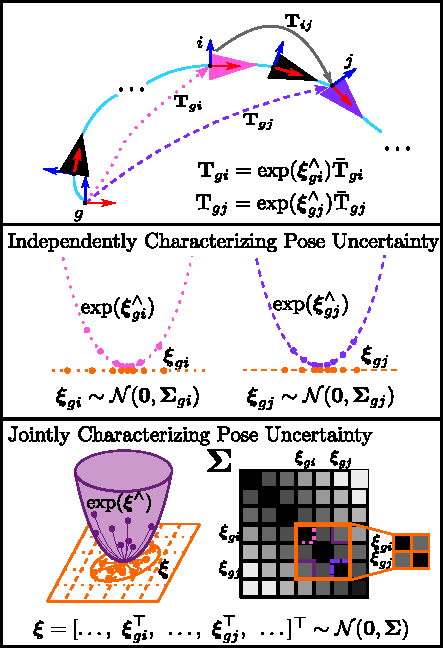
\includegraphics[width=0.9\columnwidth]{figures/main-example2.pdf}
    \caption{
    最先进的位姿图SLAM算法在每个时间步中估计机器人机体相对于固定坐标系的位姿(如上图中的 $i$ 和 $j$ ),分别用 $\mathbf{T}_{gi}$ 和 $\mathbf{T}_{gj}$ 表示。 
    在求解SLAM后,通常需要通过执行各种操作(如位姿组合、位姿求逆和相对位姿估计)来提取附加信息,同时精确地传播不确定性。
    本图顶部显示了一个相对位姿操作 $\mathbf{T}_{ij}$ 的示例。
    最近的研究已经表明,在特殊欧几里德群的李代数(如上图中所示)中,将不确定性作为高斯随机变量($\boldsymbol{\xi}_{gi}, \boldsymbol{\xi}_{gj}$)的刻画,会导致一致性的提高 \cite{barfoot2014associating};然而,这种方法的侧重于位姿组合,同时假设底层位姿是独立的。
    通常,从SLAM中估计的位姿高度相关 \cite{dissanayake2001a}。
    本文提出了一个在李代数空间中联合刻画一组相关位姿的不确定性的框架(如上图底部插图所示)。 
    然后描述了如何在此框架内执行位姿组合、位姿求逆和相对位姿操作。}
    \label{fig:main_example}
\end{figure}

\section{序言}

机器人位姿(位置和方向)不确定性的精确刻画对于鲁棒的长期的自主性至关重要,因为规划和安全决策通常基于它们的数值 \cite{thrun2005probabilistic}。例如,过于自信的位置估计可能导致自动驾驶汽车驶出车道或水下航行器与水下建筑相撞。另一方面,信心不足会导致行动迟缓。  

最早刻画坐标帧关系的位姿不确定性的论文之一,使用多元高斯参数向量和相关协方差矩阵来表示物体的相对位姿 \cite{smith1986a}。 
这篇论文后来被Smith、Self和Cheesman \cite{smith1990a} 扩展,将多个不确定的空间关系表示为一个可用于评估任意给定位姿相对于任意其它位姿的不确定性的随机映射(\textit{stochastic map})。 
他们还提出了几种操作(如 \figref{fig:main_example} 所示的相对位姿操作),这些操作能够提取不直接估计的附加信息,以及通过这些操作基于一阶坐标的方法传播不确定性。 
% These methods had a significant effect on the field and have been widely used since. 
为简洁起见,在文献 \cite{smith1990a} 中提出的操作通常由论文作者的首字母 (SSC) 表示。 



尽管众所周知,刚体变换(或 $\mathbb{R}^3$ 的运动群)是由三维(3D)特殊欧几里德群~\citep{spong2005robot,murray1994mathematical},$\mathrm{SE}(3)$ 描述的,这些变换的不确定性通常在局部坐标系中建模,从而导致在估计问题~\citep{huang2007convergence}中的不一致性或在不确定性传播~\citep{rodriguez2018importance}中的单调性损失。\citet{wang2008nonparametric} 和 \citet{long2013banana} 通过使用位于 $\mathrm{SE}(d)$ 的李代数中的指数坐标(\emph{exponential coordinates})来表示每个位姿,能够克服这些问题。 
 
\citet{barfoot2014associating} 证明了通过直接在李代数中对不确定性进行建模,然后使用指数映射在群空间中诱导分布,可以简化传播计算。 
由于李代数是一个向量空间,一个小的扰动项可以在 $\mathbb{R}^6$ 中建模为零均值高斯噪声,然后用于扰动群空间中的平均(或标称)位姿。 
文献 \cite{barfoot2014associating} 然后在此基础上,推导出当相关位姿独立时位姿组合操作的一阶和二阶不确定性传播。 
我们对一组位姿的不确定性进行建模的方法与此类似,但是我们放弃了独立性要求,因为由SLAM估计的位姿很少独立,并且它还附加描述了位姿求逆和相对位姿提取的附加操作(参见 \figref{fig:main_example})。 

本文的主要贡献如下:
\begin{enumerate}
    \item 我们提出了一个框架,描述了如何表示联合相关的位姿,同时使用李代数来刻画不确定性;
    \item 我们推导了所提议的框架与SSC操作的等价性;
    \item 我们描述了如何从替代的不确定性刻画参数化转换到所提议的框架(包括从MLE的解中提取李代数协方差);而且, 
    \item 我们发布了一个配套的C++库实现,以及这里介绍的例子。
\end{enumerate}
本文的其余部分组织如下:
第 \ref{sec:SE3} 节简要介绍了特殊欧几里德群及其在李群理论中的一些必要概念。 
第 \ref{sec:SSC} 节提供了SSC不确定性表示框架及其相关操作的摘要。 
第 \ref{sec:lie_joint_uncertainty} 节描述如何使用李代数来描述联合分布位姿的不确定性。 
第 \ref{sec:pose_composition}, \secref{sec:inverse}, 和 \secref{sec:relative_pose} 节分别描述了位姿组合、位姿求逆和相对位姿操作的推导,以及在李代数上不确定性的刻画。
第 \ref{sec:conversion} 节描述了如何从基于坐标系的不确定性表示转换为基于李代数的不确定性表示,以及如何从MLE的解中提取位姿不确定性的估计。
第 \ref{sec:eval} 节描述了所提议的方法的实验评估。
第 \ref{sec:library} 节描述了已发布的代码库的实现。 
最后, 第 \ref{sec:conclusion} 节总结全文。 



\section{\normalfont\bfseries 数学预备知识 \label{sec:Mathematical-Preliminaries}}

对偶四元数 \cite{Selig2005} 是以下集合的元素
\begin{align}
\mathcal{H} & \triangleq\{\quat h_{\mathcal{P}}+\dual\quat h_{\mathcal{D}}\::\:\quat h_{\mathcal{P}},\quat h_{\mathcal{D}}\in\mathbb{H},\,\dual\neq0,\,\dual^{2}=0\},\label{eq:dq_def}
\end{align}
其中
\begin{align}
\mathbb{H} & \triangleq\{h_{1}+\imi h_{2}+\imj h_{3}+\imk h_{4}\::\:h_{1},h_{2},h_{3},h_{4}\in\mathbb{R}\}\label{eq:quat_def}
\end{align}
是四元数的集合,其中 $\imi$,$\imj$ 和 $\imk$ 是虚数单位,具有性质 $\imi^{2}=\imj^{2}=\imk^{2}=\imi\imj\imk=-1$\cite{Hamilton1844}。
对偶四元数的加法和乘法类似于实数和复数的对应物。人们必须只遵从对偶单位 $\dual$ 和虚数单位 $\imi,\imj,\imk$ 的性质。

给定 $\dq h\in\mathcal{H}$ 使得
\[
\dq h=\underbrace{h_{1}+\imi h_{2}+\imj h_{3}+\imk h_{4}}_{\quat h_{\mathcal{P}}}+\dual\underbrace{\left(h_{5}+\imi h_{6}+\imj h_{7}+\imk h_{8}\right)}_{\quat h_{\mathcal{D}}},
\]
算子 $\mathcal{P}\left(\dq h\right)\triangleq\quat h_{\mathcal{P}}$
和 $\mathcal{D}\left(\dq h\right)\triangleq\quat h_{\mathcal{D}}$
分别提供 $\dq h$ 的原生部分和对偶部分,
而算子 $\real{\dq h}\triangleq h_{1}+\dual h_{5}$
和 $\imag{\dq h}=\imi h_{2}+\imj h_{3}+\imk h_{4}+\dual\left(\imi h_{6}+\imj h_{7}+\imk h_{8}\right)$
分别提供 $\dq h$ 的实数和虚数部分。
$\dq h$ 的共轭被定义为 $\dq h^{*}\triangleq\real{\dq h}-\imag{\dq h}$,
并且其范数给出为 $\norm{\dq h}=\sqrt{\dq h\dq h^{*}}=\sqrt{\dq h^{*}\dq h}$。

单位对偶四元数的子集 $\dq{\mathcal{S}}=\left\{ \dq h\in\mathcal{H}:\norm{\dq h}=1\right\} $ 用于表示三维空间中的位姿(位置和方向),并在乘法运算下形成群 $\spinr$。\footnote{符号 $\ltimes$ 表示群之间的半直接乘积
\cite[p. 22]{Selig2005}。} 任意 $\dq x\in\dq{\mathcal{S}}$ 总是可以写为 $\dq x=\quat r+\dual\left(1/2\right)\quat p\quat r$,其中 $\quat p=\imi x+\imj y+\imk z$ 代表三维空间中的位置 $\left(x,y,z\right)$,并且 $\quat r=\cos\left(\phi/2\right)+\quat n\sin\left(\phi/2\right)$ 代表一个旋转,在其中 $\phi\in[0,2\pi)$ 是围绕旋转轴 $\quat n\in\mathbb{H}_{p}\cap\mathbb{S}^{3}$ 的旋转角度,其中 $\mathbb{H}_{p}\triangleq\left\{ \quat h\in\mathbb{H}:\real{\quat h}=0\right\} $ 并且 $\mathbb{S}^{3}=\left\{ \quat h\in\mathbb{H}:\norm{\quat h}=1\right\} $\cite{Selig2005}。

给定纯对偶四元数集合 $\mathcal{H}_{p}=\left\{ \dq h\in\mathcal{H}:\real{\dq h}=0\right\}$,其被用于表示运动旋量(twist)和动力旋量(wrenche),算子 $\mathrm{Ad}:\dq{\mathcal{S}}\times\mathcal{H}_{p}\to\mathcal{H}_{p}$ 在这些实体上执行刚体运动。例如,给定在帧 $\frame a$ 中表达的运动旋量,即 $\dq{\xi}^{a}\in\mathcal{H}_{p}$,以及单位对偶四元数 $\dq x_{a}^{b}$,其给出 $\frame a$ 相对于 $\frame b$ 的位姿,同样的运动旋量在帧 $\frame b$ 中表达为\footnote{注意,上标表示原始帧,而下标表示已修改的帧。本文始终保持下标和上标的约定。如果没有使用上标,我们就假定是全局惯性帧。}
\begin{equation}
\dq{\xi}^{b}=\ad{\dq x_{a}^{b}}{\dq{\xi}^{a}}=\dq x_{a}^{b}\dq{\xi}^{a}\left(\dq x_{a}^{b}\right)^{*}.\label{eq:adj_transf}
\end{equation}

$\dq x_{b}^{a}$ 的时间导数由文献 \cite{Adorno2017} 给出为
\begin{equation}
\dot{\dq x}_{b}^{a}=\frac{1}{2}\dq{\xi}_{ab}^{a}\dq x_{b}^{a}=\frac{1}{2}\dq x_{b}^{a}\dq{\xi}_{ab}^{b},\label{eq:x_dot}
\end{equation}
其中 
\begin{gather}
\dq{\xi}_{ab}^{a}=\quat{\omega}_{ab}^{a}+\dual\left(\dot{\quat p}_{ab}^{a}+\quat p_{ab}^{a}\times\quat{\omega}_{ab}^{a}\right)\label{eq:twist-inertial-frame}
\end{gather}
是帧 $\frame b$ 相对于帧 $\frame a$ 的运动旋量,在帧 $\frame a$ 中表达,\footnote{在这里使用三个索引很重要,因为从第三帧可以看到两个帧之间的运动旋量。因此,例如,$\dq{\xi}_{a,b}^{c}$ 是帧 $\frame b$ 相对于帧 $\frame a$ 的运动旋量,在帧 $\frame c$ 中表达。同样的解释也被用于动力旋量,这将在第~\ref{subsec:dqNE_backward_recursion} 节中适当介绍。} 其中 $\quat{\omega}_{ab}^{a}\in\mathbb{H}_{p}$ 是角速度,并且
\begin{gather}
\dq{\xi}_{ab}^{b}=\ad{\dq x_{a}^{b}}{\dq{\xi}_{ab}^{a}}=\quat{\omega}_{ab}^{b}+\dual\dot{\quat p}_{ab}^{b}\label{eq:twist-body-frame}
\end{gather}
是在 $\frame b$ 中表达的运动旋量。而且,$\dq{\xi}_{ab}^{a}$ 和 $\dq{\xi}_{ab}^{b}$ 是与 $\spinr$ 相关联的李代数的元素。另外,
\begin{align}
\quat p\times\quat{\omega}\triangleq & \frac{\quat p\quat{\omega}-\quat{\omega}\quat p}{2},\label{eq:cross_product}
\end{align}
$\quat p,\quat{\omega}\in\mathbb{H}_{p}$,是纯四元数之间的交叉积,类似于在 $\mathbb{R}^{3}$ 中向量之间的交叉积 \cite{Adorno2017}。

$\dq l,\dq s\in\mathcal{H}_{p}$ 之间的叉积,其中
$\dq l=\quat l+\dual\quat l'$ 和 $\dq s=\quat s+\dual\quat s'$,
类似于方程 \eqref{eq:cross_product} 并给出为
\begin{equation}
\dq l\times\dq s\triangleq\frac{\dq l\dq s-\dq s\dq l}{2}=\quat l\times\quat s+\dual\left(\quat l\times\quat s'+\quat l'\times\quat s\right).\label{eq:cross_product_dq}
\end{equation}

\begin{lemma}\label{lem:derivative_of_adjoint_transformation}

如果 $\dq x\in\mathcal{\dq S}$,使得 $\dot{\dq x}=(1/2)\dq{\xi}\dq x$
并且 $\dq{\xi}'\in\mathcal{H}_{p}$,则
\begin{equation}
\frac{d}{dt}\left(\ad{\dq x}{\dq{\xi}'}\right)=\ad{\dq x}{\dot{\dq{\xi}'}}+\dq{\xi}\times\left(\ad{\dq x}{\dq{\xi}'}\right).\label{eq:derivative_of_adjoint_transformation}
\end{equation}

\end{lemma}

\begin{proof}

使用方程 \eqref{eq:adj_transf},方程 \eqref{eq:x_dot},以及以下事实
$\left(\dq{\xi}\dq x\right)^{*}=-\dq x^{*}\dq{\xi}$,我们获得
\begin{align}
\frac{d}{dt}\left(\ad{\dq x}{\dq{\xi}}'\right) & =\dot{\dq x}\dq{\xi}'\dq x^{*}+\dq x\dot{\dq{\xi}'}\dq x^{*}+\dq x\dq{\xi}'\dot{\dq x}^{*}\nonumber \\
 & =\frac{1}{2}\dq{\xi}\left(\dq x\dq{\xi}'\dq x^{*}\right)+\dq x\dot{\dq{\xi}'}\dq x^{*}-\frac{1}{2}\left(\dq x\dq{\xi}'\dq x^{*}\right)\dq{\xi}.\label{eq:adjoint_derivative_intermediate}
\end{align}
最后,在方程 \eqref{eq:adjoint_derivative_intermediate} 中使用方程 \eqref{eq:cross_product_dq} 得到方程 \eqref{eq:derivative_of_adjoint_transformation}。

\end{proof}

四元数惯性张量被定义为
\begin{equation}
\quat{\mathbb{I}}\triangleq\left(\quat i_{x},\quat i_{y},\quat i_{z}\right)\in\mathbb{H}_{p}^{3}\subset\mathcal{H}^{n},\label{eq:quat_inertia_tensor}
\end{equation}
其中 $\quat i_{x}=I_{xx}\imi+I_{xy}\imj+I_{xz}\imk$,$\quat i_{y}=I_{yx}\imi+I_{yy}\imj+I_{yz}\imk$,
以及 $\quat i_{z}=I_{zx}\imi+I_{zy}\imj+I_{zz}\imk$,这其中 $I_{nn}$,
其中 $n\in\left\{ x,y,z\right\} $,是刚体的惯性张量的元素。

\begin{definition}\label{def_operator_l}

给定 $\quat A=\left(\quat a_{x},\quat a_{y},\quat a_{z}\right)\in\mathbb{H}_{p}^{3}$
和 $\quat b\in\mathbb{H}_{p}$,算子 $\mathcal{L}_{3}:\mathbb{H}_{p}^{3}\times\mathbb{H}_{p}\to\mathbb{H}_{p}$,
被定义为
\begin{align}
\mathcal{L}_{3}\left(\quat A\right)\quat b & =\imi\dotproduct{\quat a_{x},\quat b}+\imj\dotproduct{\quat a_{y},\quat b}+\imk\dotproduct{\quat a_{z},\quat b},\label{eq:operator_l}
\end{align}
其中 $\dotproduct{\cdot,\cdot}:\mathbb{H}_{p}\to\mathbb{R}$ 是四元数之间的内积;\footnote{在 $\mathbb{H}_{p}$ 中的内积等同于在 $\mathbb{R}^{3}$ 中的内积。} 也就是,给定 $\quat a,\quat b\in\mathbb{H}_{p}$,则 $\dotproduct{\quat a,\quat b}\triangleq-(\quat{ab}+\quat{ba})/2$。

\end{definition}

根据定义~\ref{def_operator_l},可以得出在(对偶)四元数代数中的角动量 $\quat{\ell}$,给出为
\begin{equation}
\quat{\ell}=\mathcal{L}_{3}\left(\quat{\mathbb{I}}\right)\quat{\omega},\label{eq:angular_momentum}
\end{equation}
其中 $\quat{\omega}\in\mathbb{H}_{p}$ 是角速度。直接计算表明方程 \eqref{eq:angular_momentum} 等价于向量代数中的对应项。

给定刚体的四元数惯性张量 $\quat{\mathbb{I}}'\in\mathbb{H}_{p}^{3}$,在帧 $\frame{}'$ 中表达,并且刚体的角速度 $\quat{\omega}\in\mathbb{H}_{p}$ 在 $\frame{}$ 帧中表达,在 $\frame{}$ 帧中表达的角动量给出为
\begin{equation}
\quat{\ell}=\ad{\quat r^{*}}{\mathcal{L}_{3}\left(\quat{\mathbb{I}}'\right)\ad{\quat r}{\quat{\omega}}},\label{eq:similarity-transformation}
\end{equation}
其中 $\quat r$ 是从 $\frame{}^{'}$ 到 $\frame{}$ 的旋转四元数。方程~\eqref{eq:similarity-transformation} 类似于当在 $\mathbb{R}^{3}$ 中使用旋转矩阵和向量的相似性变换时获得的方程。


\selectlanguage{american}%

\section{\normalfont\bfseries 对偶四元数牛顿-欧拉模型 \label{sec:Newton-Euler-Model}}

本节对于具有任意关节的移动机械臂,介绍使用对偶四元数代数的牛顿-欧拉模型的递归关系,假设使用对偶四元数表示的完整运动学模型是可用的 \cite{Adorno2011}。

为了说明目的,在不丧失一般性的情况下,考虑图~\ref{fig:mobile_nDOF_robot} 所示的移动机械臂,其由一个 $n_{\ell}$ 自由度的串联机械臂组成,附着到一个$3$自由度的移动基座。目标是在给定相应的机器人位形、广义速度和广义加速度的情况下,找到作用于机器人移动基座和 $n_{\ell}$ 连杆的 $n=n_{\ell}+1$ 质心(centers of mass, CoM)上的动力旋量 $\dq{\Gamma}\in\mathcal{H}_{p}^{n}$。这可以看作是一个函数 $\mathcal{N}\,:\,\mathbb{R}^{n_{\ell}+3}\times\mathbb{R}^{n_{\ell}+3}\times\mathbb{R}^{n_{\ell}+3}\rightarrow\mathcal{H}_{p}^{n}$,其中 $n_{\ell}+3$ 是位形空间的维度,并且 $n$ 是运动链中刚体的数量(例如,移动基座和连杆),使得
\begin{equation}
\dq{\Gamma}=\mathcal{N}\left(\myvec q,\dot{\myvec q},\ddot{\myvec q}\right).\label{eq:dq_NE_as_a_function}
\end{equation}
\begin{figure}[t]
\def\svgwidth{2.5\columnwidth}
\noindent \begin{centering}
{\Huge{}\resizebox{0.8\columnwidth}{!}{\input{Images/mobile_nDOF_robot.pdf_tex}}}{\Huge\par}
\par\end{centering}
\caption{一个 $n_{\ell}$ 自由度的串联机械臂的移动机械臂组合,附着到一个$3$自由度的移动基座上。\label{fig:mobile_nDOF_robot}}
\end{figure}


\subsection{\normalfont\bfseries 正向递归\label{subsec:Forward-Recursion}}

该算法的第一个过程包括机器人运动学结构的串行扫描,以计算每个质心的运动旋量。
\footnote{此后,我们将使用“质心的运动旋量”这一表达作为“附着到质心的帧的运动旋量”的简写。} 其目标是找到正向递归关系,然后使用该关系迭代地获得作用于机器人移动基座和关节的动力旋量。

\subsubsection{\normalfont\bfseries 运动旋量 \label{subsec:Twists}}

移动基座的质心(即,串联运动链中的第一个质心)相对于惯性帧 $\frame 0$ 的运动旋量,在帧 $\frame{c_{1}}$ 中表达,由纯对偶四元数给出为
\begin{align}
\dq{\xi}_{0,c_{1}}^{c_{1}} & =\quat{\omega}_{0,c_{1}}^{c_{1}}+\dual\quat v_{0,c_{1}}^{c_{1}},\label{eq:twist_c1_0}
\end{align}
其中 $\quat{\omega}_{0,c_{1}}^{c_{1}}=\omega_{x}\imi+\omega_{y}\imj+\omega_{z}\imk$
和 $\quat v_{0,c_{1}}^{c_{1}}=v_{x}\imi+v_{y}\imj+v_{z}\imk$ 分别是
角速度和线速度。一个完整移动基座的运动旋量在运动学上等效于一个平面关节的运动旋量,如表~\ref{tab:joint_twists-2} 所示。

第一个连杆质心(即串联运动链中的第二个刚体的质心)相对于惯性帧的运动旋量不仅取决于其关节产生的运动旋量,还取决于移动基座的运动旋量,因为它们是物理附着的。因此,
\begin{align}
\dq{\xi}_{0,c_{2}}^{c_{2}} & =\dq{\xi}_{0,j_{1}}^{c_{2}}+\dq{\xi}_{j_{1},c_{2}}^{c_{2}},\nonumber \\
 & =\ad{\dq x_{c_{1}}^{c_{2}}}{\dq{\xi}_{0,j_{1}}^{c_{1}}}+\ad{\dq x_{j_{1}}^{c_{2}}}{\dq{\xi}_{j_{1},c_{2}}^{j_{1}}},\nonumber \\
 & =\ad{\dq x_{c_{1}}^{c_{2}}}{\left(\dq{\xi}_{0,c_{1}}^{c_{1}}+\dq{\xi}_{c_{1},j_{1}}^{c_{1}}\right)}+\ad{\dq x_{j_{1}}^{c_{2}}}{\dq{\xi}_{j_{1},c_{2}}^{j_{1}}},\label{eq:twist_c2_0}
\end{align}
其中 $\dq{\xi}_{j_{1},c_{2}}^{j_{1}}=\quat{\omega}_{j_{1},c_{2}}^{j_{1}}+\dual\quat v_{j_{1},c_{2}}^{j_{1}}$
是在 $\frame{c_{2}}$ 上由第一个关节产生的运动旋量,并且 $\dq{\xi}_{0,j_{1}}^{c_{2}}$ 是在 $\frame{j_{1}}$ 上由移动基座产生的运动旋量,但使用合适的变换,如方程 \eqref{eq:adj_transf},在 $\frame{c_{2}}$ 中表达。表~\ref{tab:joint_twists-2} 对于不同类型的关节列出了它们的运动旋量,其中 $\quat l\in\mathbb{H}_{p}\cap\mathbb{S}^{3}$ 是一个常量(\emph{constant})单位范数纯四元数,其等价于R3中的一个向量,用于定义一个任意轴。例如,当使用 Denavit-Hartenberg (DH) 约定时,$\quat l=\imk$,这等价于 $z$ 轴。此外,$\omega,\omega_{x},\omega_{y},\omega_{z}\in\mathbb{R}$ 和 $v,v_{x},v_{y},v_{z}\in\mathbb{R}$ 分别是角速度和线速度的标量分量。同样,当使用DH约定时,对于旋转关节 $\omega=\dot{\theta}$,并且对于棱柱状关节 $v=\dot{d}$。对于螺旋关节,常量 $h\in\mathbb{R}$ 被称为旋距(\emph{pitch})。

\begin{table*}[t]
\begin{centering}
\caption{在机器人中一些最常用的关节的扭曲,其中
$\protect\quat l\in\mathbb{H}_{p}\cap\mathbb{S}^{3}$ 并且 $\omega,\omega_{x},\omega_{y},\omega_{z},v,v_{x},v_{y},v_{z},h\in\mathbb{R}$。\label{tab:joint_twists-2}}
\par\end{centering}
\centering{}%
\begin{tabular}{>{\centering}p{3.3cm}>{\centering}m{2.2cm}>{\centering}p{2.5cm}>{\centering}p{3cm}>{\centering}p{2.5cm}>{\centering}p{2.5cm}c}
\hline 
\noindent \centering{}$6$自由度关节 & \noindent \centering{}旋转关节 & \noindent \centering{}球面关节 & \noindent \centering{}圆柱关节 & \noindent \centering{}平面关节 & \noindent \centering{}棱柱关节 & 螺旋关节\tabularnewline
\hline 
\noindent \centering{}\resizebox{0.22\columnwidth}{!}{\input{Images/joints/6DOF.pdf_tex}} & \noindent \centering{}\resizebox{0.15\columnwidth}{!}{\input{Images/joints/rotational.pdf_tex}} & \noindent \centering{}\resizebox{0.18\columnwidth}{!}{\input{Images/joints/spherical.pdf_tex}} & \noindent \centering{}\resizebox{0.15\columnwidth}{!}{\input{Images/joints/cylindrical.pdf_tex}} & \noindent \centering{}\resizebox{0.18\columnwidth}{!}{\input{Images/joints/planar.pdf_tex}} & \noindent \centering{}\resizebox{0.13\columnwidth}{!}{\input{Images/joints/prismatic.pdf_tex}} & \resizebox{0.2\columnwidth}{!}{\input{Images/joints/screw.pdf_tex}}\tabularnewline
\hline 
\multirow{2}{3.3cm}{\noindent \centering{}$\dq{\xi}=\omega_{x}\imi+\omega_{y}\imj+\omega_{z}\imk+\dual\left(v_{x}\imi+v_{y}\imj+v_{z}\imk\right)$} & \multirow{2}{2.2cm}{\noindent \centering{}$\dq{\xi}=\omega\quat l$} & \multirow{2}{2.5cm}{\noindent \centering{}$\dq{\xi}=\omega_{x}\imi+\omega_{y}\imj\allowbreak+\omega_{z}\imk$} & \multirow{2}{3cm}{\noindent \centering{}$\dq{\xi}=\left(\omega+\dual v\right)\quat l$} & \multirow{2}{2.5cm}{\noindent \centering{}$\dq{\xi}=\omega\quat l+\allowbreak\dual\left(v_{x}\imi+v_{y}\imj\right)$} & \multirow{2}{2.5cm}{\noindent \centering{}$\dq{\xi}=\dual v\quat l$} & \multirow{2}{*}{$\dq{\xi}=\left(\omega+\dual h\omega\right)\quat l$}\tabularnewline
 &  &  &  &  &  & \tabularnewline
\hline 
\end{tabular}
\end{table*}

此外,$\dq{\xi}_{c_{1},j_{1}}^{c_{1}}=0$,因为 $\dot{\dq x}_{j_{1}}^{c_{1}}=0$。因此,
\begin{align*}
\dq{\xi}_{0,c_{2}}^{c_{2}} & =\ad{\dq x_{c_{1}}^{c_{2}}}{\dq{\xi}_{0,c_{1}}^{c_{1}}}+\ad{\dq x_{j_{1}}^{c_{2}}}{\dq{\xi}_{j_{1},c_{2}}^{j_{1}}}.
\end{align*}
而且,展开 $\ad{\dq x_{j_{1}}^{c_{2}}}{\dq{\xi}_{j_{1},c_{2}}^{j_{1}}}$,我们获得
\[
\ad{\dq x_{j_{1}}^{c_{2}}}{\dq{\xi}_{j_{1},c_{2}}^{j_{1}}}=\quat{\omega}_{j_{1},c_{2}}^{c_{2}}+\dual\left(\quat v_{j_{1},c_{2}}^{c_{2}}+\quat{\omega}_{j_{1},c_{2}}^{c_{2}}\times\quat p_{j_{1},c_{2}}^{c_{2}}\right),
\]
其中因为在从质心处(即从 $\frame{j_{1}}$ 处)移位的一个点中应用角速度而产生的线速度以代数方式产生。图~\ref{fig:intuition_twist_transf} 说明了使用纯旋转关节时的这种现象(即 $\dq{\xi}_{j_{i},c_{i+1}}^{j_{i}}=\quat{\omega}_{j_{i},c_{i+1}}^{j_{i}}=\omega_{i}\myvec n_{j_{i},c_{i+1}}^{j_{i}}$,其中 $\myvec n_{j_{i},c_{i+1}}^{j_{i}}\in\mathbb{H}_{p}\cap\mathbb{S}^{3}$ 是一个任意的单位范数旋转轴)。

\begin{figure*}[t]
\def\svgwidth{2.0\columnwidth}
\begin{centering}
{\huge{}\scalebox{0.5}[0.5]{\input{Images/intuition_twist_transf.pdf_tex}}}{\huge\par}
\par\end{centering}
\caption{运动旋量 $\protect\dq{\xi}_{j_{i},c_{i+1}}^{c_{i+1}}$ 由于围绕参考帧 $\protect\frame{j_{i}}$ 的一个任意轴施加角速度 $\omega_{i}$ 而产生。$\protect\frame{c_{i+1}}$ 所遵循的圆形轨迹由灰色虚线表示。$\omega_{i}$ 的应用导致的线速度通过伴随变换以代数方式出现。因此,参考帧 $\protect\frame{c_{i+1}}$ 的切向速度,以黑色实线箭头表示,由运动旋量 $\protect\dq{\xi}_{j_{i},c_{i+1}}^{c_{i+1}}$ 的对偶部分给出。 \label{fig:intuition_twist_transf}}
\end{figure*}

更一般地,在 $\frame{c_{i}}$ 中的运动旋量,其提供 $\frame{c_{i}}$ 相对于 $\frame 0$ 的运动,产生于运动链中的前 $i$ 个刚体的运动,给出为
\begin{align}
\dq{\xi}_{0,c_{i}}^{c_{i}} & =\dq{\xi}_{0,j_{i-1}}^{c_{i}}+\dq{\xi}_{j_{i-1},c_{i}}^{c_{i}}\label{eq:twist_ci_0}
\end{align}
其中 $\dq{\xi}_{0,j_{i-1}}^{c_{i}}$ 是与前 $i-1$ 个刚体的运动相关的运动旋量,并且 $\dq{\xi}_{j_{i-1},c_{i}}^{c_{i}}$ 是与第 $i$ 个刚体的运动相关的运动旋量。另外,对于任意 $a$,$\dq{\xi}_{0,0}^{a}=0$。

分析方程 \eqref{eq:twist_c1_0},\eqref{eq:twist_c2_0} 和 \eqref{eq:twist_ci_0},通过归纳,我们发现,第 $i$ 个质心总的运动旋量的递归关系,其具有直到第 $i$ 个刚体的所有刚体的贡献,在 $\frame{c_{i}}$ 中表达,为
\begin{multline*}
\dq{\xi}_{0,c_{i}}^{c_{i}}=\ad{\dq x_{c_{i-1}}^{c_{i}}}{\left(\dq{\xi}_{0,c_{i-1}}^{c_{i-1}}+\dq{\xi}_{c_{i-1},j_{i-1}}^{c_{i-1}}\right)}\\
+\ad{\dq x_{j_{i-1}}^{c_{i}}}{\dq{\xi}_{j_{i-1},c_{i}}^{j_{i-1}}},
\end{multline*}
其中 $c_{0}=j_{0}=0$,并且 $\dq{\xi}_{c_{i-1},j_{i-1}}^{c_{i-1}}=0$,因为对于所有的 $i$,$\dot{\dq x}_{j_{i-1}}^{c_{i-1}}=0$ 。因此,

\begin{equation}
\dq{\xi}_{0,c_{i}}^{c_{i}}=\ad{\dq x_{c_{i-1}}^{c_{i}}}{\dq{\xi}_{0,c_{i-1}}^{c_{i-1}}}+\ad{\dq x_{j_{i-1}}^{c_{i}}}{\dq{\xi}_{j_{i-1},c_{i}}^{j_{i-1}}.}\label{eq:twist_rec}
\end{equation}
由于运动旋量 $\dq{\xi}_{j_{i-1},c_{i}}^{j_{i-1}}$ 是由第 $i$ 个关节产生的,其表达方式取决于第 $i$ 个关节是哪种类型(\emph{参见}表~\ref{tab:joint_twists-2})。类似地,运动旋量 $\dq{\xi}_{0,c_{1}}^{c_{1}}$ 取决于移动基座是哪种类型(例如,对于完整移动基座,它等效于平面关节给出的运动旋量)。变换 $\dq x_{c_{i-1}}^{c_{i}}$ 被计算为 $\dq x_{c_{i-1}}^{c_{i}}=\left(\dq x_{c_{i}}^{0}\right)^{*}\dq x_{c_{i-1}}^{0}$,其中当 $\dq x_{0}^{0}=1$ 时,$\dq x_{c_{i}}^{0}=\dq x_{c_{i-1}}^{0}\dq x_{j_{i-1}}^{c_{i-1}}\dq x_{c_{i}}^{j_{i-1}}$,变换 $\dq x_{j_{i-1}}^{c_{i-1}}$ 为常量,并且 $\dq x_{c_{i}}^{j_{i-1}}$ 是第 $\left(i-1\right)$ 个关节(或 $i=1$ 时的移动基座)的参数的函数。

\subsubsection{\normalfont\bfseries 运动旋量的时间导数 \label{subsec:time_derivative_twists}}

方程 \eqref{eq:twist_rec} 的时间导数,我们使用方程 \eqref{eq:derivative_of_adjoint_transformation} 来获得
\begin{multline*}
\dot{\dq{\xi}}_{0,c_{i}}^{c_{i}}=\ad{\dq x_{c_{i-1}}^{c_{i}}}{\dot{\dq{\xi}}_{0,c_{i-1}}^{c_{i-1}}}\\
+\dq{\xi}_{c_{i},c_{i-1}}^{c_{i}}\times\left(\ad{\dq x_{c_{i-1}}^{c_{i}}}{\dq{\xi}_{0,c_{i-1}}^{c_{i-1}}}\right)+\ad{\dq x_{j_{i-1}}^{c_{i}}}{\dot{\dq{\xi}}_{j_{i-1},c_{i}}^{j_{i-1}}}\\
+\dq{\xi}_{c_{i},j_{i-1}}^{c_{i}}\times\left(\ad{\dq x_{j_{i-1}}^{c_{i}}}{\dq{\xi}_{j_{i-1},c_{i}}^{j_{i-1}}}\right).
\end{multline*}
由于 $\dq{\xi}_{j_{i-1},c_{i}}^{c_{i}}=-\dq{\xi}_{c_{i},j_{i-1}}^{c_{i}}$
则
\[
\dq{\xi}_{c_{i},j_{i-1}}^{c_{i}}\times\left(\ad{\dq x_{j_{i-1}}^{c_{i}}}{\dq{\xi}_{j_{i-1},c_{i}}^{j_{i-1}}}\right)=-\dq{\xi}_{c_{i},j_{i-1}}^{c_{i}}\times\dq{\xi}_{c_{i},j_{i-1}}^{c_{i}}=0.
\]
因此,

\begin{multline}
\dot{\dq{\xi}}_{0,c_{i}}^{c_{i}}=\ad{\dq x_{c_{i-1}}^{c_{i}}}{\dot{\dq{\xi}}_{0,c_{i-1}}^{c_{i-1}}}+\ad{\dq x_{j_{i-1}}^{c_{i}}}{\dot{\dq{\xi}}_{j_{i-1},c_{i}}^{j_{i-1}}}\\
+\dq{\xi}_{c_{i},c_{i-1}}^{c_{i}}\times\left[\ad{\dq x_{c_{i-1}}^{c_{i}}}{\dq{\xi}_{0,c_{i-1}}^{c_{i-1}}}\right],\label{eq:twist_dot_rec}
\end{multline}
其中 $\dot{\dq{\xi}}_{0,c_{0}}^{c_{0}}\triangleq0$。另外,由于
$\dq{\xi}_{c_{i},c_{i-1}}^{j_{i-1}}=\dq{\xi}_{c_{i},j_{i-1}}^{j_{i-1}}+\dq{\xi}_{j_{i-1},c_{i-1}}^{j_{i-1}}$
并且 $\dq{\xi}_{j_{i-1},c_{i-1}}^{j_{i-1}}=0$,则
\begin{align}
\dq{\xi}_{c_{i},c_{i-1}}^{c_{i}} & =\ad{\dq x_{j_{i-1}}^{c_{i}}}{\dq{\xi}_{c_{i},j_{i-1}}^{j_{i-1}}}=-\ad{\dq x_{j_{i-1}}^{c_{i}}}{\dq{\xi}_{j_{i-1},c_{i}}^{j_{i-1}}}.\label{eq:twists_between_adjacent_CoM}
\end{align}

如第~\ref{subsec:Twists} 节所示,运动旋量 $\dq{\xi}_{j_{i-1},c_{i}}^{j_{i-1}}$ 取决于第 $i$ 个关节的类型,并因此,这个项 $\dot{\dq{\xi}}_{j_{i-1},c_{i}}^{j_{i-1}}$ 也是如此。例如,如果第 $i$ 个关节是旋转的,则 $\dot{\dq{\xi}}_{j_{i-1},c_{i}}^{j_{i-1}}=\dot{\omega}_{i}\quat l_{j_{i}}^{j_{i}}$。如果它是棱形的,则 $\dot{\dq{\xi}}_{j_{i-1},c_{i}}^{j_{i-1}}=\dual\dot{v}_{i}\quat l_{j_{i}}^{j_{i}}$。类似地,如果它是螺旋形的,则 $\dot{\dq{\xi}}_{j_{i-1},c_{i}}^{j_{i-1}}=\left(\dot{\omega}_{i}+\dual h\dot{\omega}_{i}\right)\quat l_{j_{i}}^{j_{i}}$,如此等等。同样的推理适用于移动基座的运动旋量 $\dot{\dq{\xi}}_{0,c_{1}}^{c_{1}}$。

\selectlanguage{english}%

\selectlanguage{american}%
\begin{remark}

尽管方程 \eqref{eq:twist_dot_rec} 是以递归形式编写的,但我们始终可以如在方程 \eqref{eq:twist-inertial-frame} 和 \eqref{eq:twist-body-frame} 中的那样将运动旋量写出来。因此,由于 $\dq{\xi}_{0,c_{i}}^{c_{i}}=\ad{\dq x_{0}^{c_{i}}}{\dq{\xi}_{0,c_{i}}^{0}}$,其中 $\dq{\xi}_{0,c_{i}}^{0}=\quat{\omega}_{0,c_{i}}^{0}+\dual(\dot{\quat p}_{0,c_{i}}^{0}+\quat p_{0,c_{i}}^{0}\times\quat{\omega}_{0,c_{i}}^{0})$,我们使用方程 \eqref{eq:derivative_of_adjoint_transformation} 以获得
\begin{align}
\dot{\dq{\xi}}_{0,c_{i}}^{c_{i}} & {=}\ad{\dq x_{0}^{c_{i}}}{\dot{\dq{\xi}}_{0,c_{i}}^{0}{=}\dot{\quat{\omega}}_{0,c_{i}}^{c_{i}}{+}\dual\left(\ddot{\quat p}_{0,c_{i}}^{c_{i}}{+}\dot{\quat p}_{0,c_{i}}^{c_{i}}{\times}\quat{\omega}_{0,c_{i}}^{c_{i}}\right)}\label{eq:twist_derivative_explicit_form}
\end{align}
 因为 $\dq{\xi}_{c_{i},0}^{c_{i}}\times\ad{\dq x_{0}^{c_{i}}}{\dq{\xi}_{0,c_{i}}^{0}}=-\dq{\xi}_{0,c_{i}}^{c_{i}}\times\dq{\xi}_{0,c_{i}}^{c_{i}}=0$。
由于 $\getd{\dot{\dq{\xi}}_{0,c_{i}}^{c_{i}}}=\ddot{\quat p}_{0,c_{i}}^{c_{i}}+\dot{\quat p}_{0,c_{i}}^{c_{i}}\times\quat{\omega}_{0,c_{i}}^{c_{i}}$
则
\begin{gather}
\ddot{\quat p}_{0,c_{i}}^{c_{i}}=\getd{\dot{\dq{\xi}}_{0,c_{i}}^{c_{i}}}-\getd{\dq{\xi}_{0,c_{i}}^{c_{i}}}\times\getp{\dq{\xi}_{0,c_{i}}^{c_{i}}}.\label{eq:linear-acceleration}
\end{gather}

\end{remark}

\subsection{\normalfont\bfseries 逆向递归\label{subsec:dqNE_backward_recursion}}

迭代算法的第二个过程是将串联机器人从最后一个刚体扫描到第一个刚体,以计算施加在每个刚体上的动力旋量。对于机器人手臂,我们对每个关节的动力旋量感兴趣,而对于移动基座,我们想找到其质心处的动力旋量。为了这个目的,我们使用在第~\ref{subsec:Forward-Recursion} 节中获得的运动旋量及其时间导数。

在获得逆向递归的一般表达式之前,让我们考虑图~\ref{fig:mobile_nDOF_robot} 中所示的移动机械臂。在第 $n_{\ell}$ 个连杆的质心处的动力旋量(即,在运动链中的第 $n$ 个质心,其中 $n=n_{\ell}+1$),在 $\frame{c_{n}}$ 中表达,由纯对偶四元数给出为

\begin{equation}
\dq{\zeta}_{0,c_{n}}^{c_{n}}=\dq{\varsigma}_{0,c_{n}}^{c_{n}}-m_{n}\quat g^{c_{n}},\label{eq:wrench_cn_in_cn}
\end{equation}
其中 $m_{n}\quat g^{c_{n}}$ 是重力分量,其中
$\quat g^{c_{n}}\in\mathbb{H}_{p}$ 是在 $\frame{c_{n}}$ 中表达的重力向量,并且 $\dq{\varsigma}_{0,c_{n}}^{c_{n}}=\quat f_{0,c_{n}}^{c_{n}}+\dual\quat{\tau}_{0,c_{n}}^{c_{n}}$,
其中 $\quat f_{0,c_{n}}^{c_{n}}=f_{x}\imi+f_{y}\imj+f_{z}\imk$
是在第 $n$ 个刚体(即第 $n_{\ell}$ 个连杆)的质心处的力,由牛顿第二定律 $\quat f_{0,c_{n}}^{c_{n}}=m_{n}\ddot{\quat p}_{0,c_{n}}^{c_{n}}$ 给出。


因此,我们使用方程 \eqref{eq:linear-acceleration} 以获得

\begin{align}
\quat f_{0,c_{n}}^{c_{n}} & =m_{n}\left(\getd{\dot{\dq{\xi}}_{0,c_{n}}^{c_{n}}}+\getp{\dq{\xi}_{0,c_{n}}^{c_{n}}}\times\getd{\dq{\xi}_{0,c_{n}}^{c_{n}}}\right).\label{eq:newton_sec_law}
\end{align}
此外,由于其角动量的变化,$\quat{\tau}_{0,c_{n}}^{c_{n}}$ 是围绕第 $n$ 个刚体的质心的扭矩,由欧拉旋转方程给出为

\begin{multline}
\quat{\tau}_{0,c_{n}}^{c_{n}}=\mathcal{L}_{3}\left(\quat{\mathbb{I}}_{n}^{c_{n}}\right)\getp{\dot{\dq{\xi}}_{0,c_{n}}^{c_{n}}}\\
+\getp{\dq{\xi}_{0,c_{n}}^{c_{n}}}\times\left(\mathcal{L}_{3}\left(\quat{\mathbb{I}}_{n}^{c_{n}}\right)\getp{\dq{\xi}_{0,c_{n}}^{c_{n}}}\right),\label{eq:euler_eq}
\end{multline}
其中 $\mathcal{L}_{3}$ 由方程 \eqref{eq:operator_l} 给出,并且 $\quat{\mathbb{I}}_{n}^{c_{n}}$
是第 $n$ 个刚体的四元数惯性张量,在其质心处表达,由方程 \eqref{eq:quat_inertia_tensor} 给出。因为方程 \eqref{eq:euler_eq} 是相对于质心计算的,所以重力加速度对扭矩没有
贡献。

在方程 \eqref{eq:wrench_cn_in_cn} 中如在方程 \eqref{eq:adj_transf} 中那样使用的伴随变换,在第 $n_{\ell}$ 个关节处的动力旋量,其由第 $n$ 个刚体的质心处的动力旋量产生,给出为:
\begin{align}
\dq{\zeta}_{0,j_{n}}^{j_{n-1}} & =\ad{\dq x_{c_{n}}^{j_{n-1}}}{\dq{\zeta}_{0,c_{n}}^{c_{n}}}.\label{eq:wrench_cn_in_jnMinus1}
\end{align}

在第 $\left(n-1\right)$ 个刚体(即,在 $\frame{c_{n-1}}$ 处)的合成动力旋量还包括来自第 $n$ 个刚体的动力旋量的影响,因为它们彼此刚性附着。因此,在第 $\left(n_{\ell}-1\right)$ 关节处(即,在 $\frame{c_{n-2}}$ 处)的合成动力旋量给出为
\begin{alignat}{1}
\dq{\zeta}_{0,j_{n-1}}^{j_{n-2}} & =\ad{\dq x_{c_{n-1}}^{j_{n-2}}}{\dq{\zeta}_{0,c_{n-1}}^{c_{n-1}}}+\ad{\dq x_{j_{n-1}}^{j_{n-2}}}{\dq{\zeta}_{0,j_{n}}^{j_{n-1}}},\label{eq:wrench_cnMinus1_in_jnMinus2}
\end{alignat}
其中 $\dq{\zeta}_{0,c_{n-1}}^{c_{n-1}}=\dq{\varsigma}_{0,c_{n-1}}^{c_{n-1}}-m_{n-1}\quat g^{c_{n-1}}$,
在其中 $\dq{\varsigma}_{0,c_{n-1}}^{c_{n-1}}=\quat f_{0,c_{n-1}}^{c_{n-1}}+\dual\quat{\tau}_{0,c_{n-1}}^{c_{n-1}}$,
是在第 $\left(n-1\right)$ 个刚体的质心处的动力旋量,在 $\frame{c_{n-1}}$ 中表达。

因此,分析方程 \eqref{eq:wrench_cn_in_cn}、\eqref{eq:wrench_cn_in_jnMinus1} 以及 \eqref{eq:wrench_cnMinus1_in_jnMinus2},我们可以发现,逆向递归关系,对于在第 $i$ 个刚体处总的动力旋量,其包括从第 $i$ 个刚体的质心的动力旋量开始,直到最后一个的质心的动力旋量,它们所有的贡献,在 $\frame{j_{i-1}}$ 中表达,为
\begin{align}
\dq{\zeta}_{0,j_{i}}^{j_{i-1}} & =\ad{\dq x_{c_{i}}^{j_{i-1}}}{\dq{\zeta}_{0,c_{i}}^{c_{i}}}+\ad{\dq x_{j_{i}}^{j_{i-1}}}{\dq{\zeta}_{0,j_{i+1}}^{j_{i}}},\label{eq:wrench_rec}
\end{align}
其中 $i\in\{1,\ldots,n\}$ 并且 $c_{0}=j_{0}=0$,这里 $\dq{\zeta}_{0,j_{n_{\ell}+2}}^{j_{n_{\ell}+1}}=\dq{\zeta}_{0,j_{n+1}}^{j_{n}}=0$
(回想这个 $n=n_{\ell}+1$) 并且 $\dq{\zeta}_{0,c_{i}}^{c_{i}}=\dq{\varsigma}_{0,c_{i}}^{c_{i}}-m_{i}\quat g^{c_{i}}$,
其中 $\dq{\varsigma}_{0,c_{i}}^{c_{i}}=\quat f_{0,c_{i}}^{c_{i}}+\dual\quat{\tau}_{0,c_{i}}^{c_{i}}$,
是在第 $i$ 个质心处的动力旋量,\footnote{如果一个\textbf{外部的}动力旋量被应用于末端操纵器,则 $\dq{\zeta}_{0,j_{n+1}}^{j_{n}}\neq0$。} $\quat f_{0,c_{i}}^{c_{i}}=m_{i}\ddot{\quat p}_{0,c_{i}}^{c_{i}}$,
并且 $\quat{\tau}_{0,c_{i}}^{c_{i}}=\mathcal{L}_{3}\left(\quat{\mathbb{I}}_{i}^{c_{i}}\right)\getp{\dot{\dq{\xi}}_{0,c_{i}}^{c_{i}}}+\getp{\dq{\xi}_{0,c_{i}}^{c_{i}}}\times\left(\mathcal{L}_{3}\left(\quat{\mathbb{I}}_{i}^{c_{i}}\right)\getp{\dq{\xi}_{0,c_{i}}^{c_{i}}}\right)$。
对于移动基座(即,在串联运动学链中的第一个质心;因此,$i=1$),注意方程 \eqref{eq:wrench_rec} 的结果为 $\dq{\zeta}_{0,j_{1}}^{j_{0}}=\ad{\dq x_{c_{1}}^{j_{0}}}{\dq{\zeta}_{0,c_{1}}^{c_{1}}}+\ad{\dq x_{j_{1}}^{j_{0}}}{\dq{\zeta}_{0,j_{2}}^{j_{1}}}$,
这意味着 $\dq{\zeta}_{0,j_{1}}^{0}=\ad{\dq x_{c_{1}}^{0}}{\dq{\zeta}_{0,c_{1}}^{c_{1}}}+\ad{\dq x_{j_{1}}^{0}}{\dq{\zeta}_{0,j_{2}}^{j_{1}}}$。

此外,变换 $\dq x_{c_{i}}^{j_{i-1}}$ 是关节或移动基座的坐标的函数。例如,移动基座的变换,$\dq x_{c_{1}}^{j_{0}}=\dq x_{c_{1}}^{0}$,取决于其坐标和旋转角度,即 $(x_{\mathrel{\mathrm{base}}},y_{\mathrel{\mathrm{base}}},\phi_{\mathrel{\mathrm{base}}})$,因此 $\dq x_{c_{1}}^{0}\triangleq\dq x_{c_{1}}^{0}(x_{\mathrel{\mathrm{base}}},y_{\mathrel{\mathrm{base}}},\phi_{\mathrel{\mathrm{base}}})$ 并且 $q_{1}=x_{\mathrel{\mathrm{base}}},q_{2}=y_{\mathrm{\mathrel{base}}},q_{3}=\phi_{\mathrm{\mathrel{base}}}$。对于具有旋转关节、棱柱关节或螺旋关节的机械臂,变换 $\dq x_{c_{i}}^{j_{i-1}}$,其中$i\geq2$,是一个仅有一个参数的函数,即 $\dq x_{c_{i}}^{j_{i-1}}\triangleq\dq x_{c_{i}}^{j_{i-1}}(q_{j_{i-1}})$。在这种情况下,$q_{j_{i-1}}=q_{i+2}$。类似地,球面和平面关节取决于三个参数,而螺旋关节取决于六个参数。因此,对于在位形向量 $\myvec q$中的每一个参数,当定义索引时必须小心。

\subsubsection{\normalfont\bfseries 特殊情况:棱柱关节与旋转关节}

在具有旋转和/或棱柱关节的机械臂的机器人中,这是最常见的情况,由方程 \eqref{eq:wrench_rec} 给出的动力旋量必须投影到关节运动轴上,通过
\begin{equation}
\dotproduct{\dq{\zeta}_{0,j_{i}}^{j_{i-1}},\quat l_{j_{i-1}}}=f_{\quat l_{i}}+\dual\tau_{\quat l_{i}},\label{eq:wrench_projection_to_motion_axis}
\end{equation}
其中 $f_{\quat l_{i}},\tau_{\quat l_{i}}\in\mathbb{R}$,并且 $\dotproduct{\dq{\zeta}_{0,j_{i}}^{j_{i-1}},\quat l_{j_{i-1}}}$
是运动旋量 $\dq{\zeta}_{0,j_{i}}^{j_{i-1}}=\quat f_{0,j_{i}}^{j_{i-1}}+\dual\quat{\tau}_{0,j_{i}}^{j_{i-1}}$ 与第 $i$ 个关节的运动轴 $\quat l_{j_{i-1}}\in\mathbb{H}_{p}\cap\mathbb{S}^{3}$ 之间的内积,给出为 \cite{Adorno2017}
\begin{align*}
\dotproduct{\dq{\zeta}_{0,j_{i}}^{j_{i-1}},\quat l_{j_{i-1}}} & =-\frac{\left(\dq{\zeta}_{0,j_{i}}^{j_{i-1}}\quat l_{j_{i-1}}+\quat l_{j_{i-1}}\dq{\zeta}_{0,j_{i}}^{j_{i-1}}\right)}{2}\\
 & =\dotproduct{\quat f_{0,j_{i}}^{j_{i-1}},\quat l_{j_{i-1}}}+\dual\dotproduct{\quat{\tau}_{0,j_{i}}^{j_{i-1}},\quat l_{j_{i-1}}}=f_{\quat l_{i}}+\dual\tau_{\quat l_{i}}.
\end{align*}
因此,如果第 $i$ 个关节是旋转关节,则相应的扭矩给出为 $\tau_{\quat l_{i}}=\getd{\dotproduct{\dq{\zeta}_{0,j_{i}}^{j_{i-1}},\quat l_{j_{i-1}}}}$。如果它是棱形关节,则沿着轴线 $\quat l_{j_{i-1}}$ 的相应的力给出为 $f_{\quat l_{i}}=\getp{\dotproduct{\dq{\zeta}_{0,j_{i}}^{j_{i-1}},\quat l_{j_{i-1}}}}$。

\subsubsection{\normalfont\bfseries 特殊情况:平面关节/完整基座}

对于具有完整移动基座和/或平面关节(运动学等效)的机器人,我们必须将动力旋量投射到关节/移动基座的所有三个运动轴上。\footnote{注意,本过程适用于所有具有一个以上运动轴的关节(例如球面关节、平面关节等等)。}也就是说,沿着关节/移动基座的 $x$ 轴和 $y$ 轴的相应的力给出为
\begin{align*}
f_{\quat l_{i_{x}}} & =\getp{\dotproduct{\dq{\zeta}_{0,j_{i}}^{j_{i-1}},\ad{\quat r_{0}^{j_{i-1}}}{\imi}}},\\
f_{\quat l_{i_{y}}} & =\getp{\dotproduct{\dq{\zeta}_{0,j_{i}}^{j_{i-1}},\ad{\quat r_{0}^{j_{i-1}}}{\imj}}},
\end{align*}
而围绕关节/移动基座的 $z$ 轴的相应扭矩给出为
\begin{align*}
\tau_{\quat l_{z}} & =\getd{\dotproduct{\dq{\zeta}_{0,j_{i}}^{j_{i-1}},\ad{\quat r_{0}^{j_{i-1}}}{\imk}}}.
\end{align*}

\selectlanguage{english}%




\section{\normalfont\bfseries 高斯最小约束原理\label{sec:Gauss-Principle}}

GPLC \cite{Kalaba1993} 是一个微分变分原理,相当于达朗贝尔原理,它基于加速度的变化。对于一个由 $n$ 个机体组成的系统,它可以被表述为最小二乘的最小化问题
\begin{gather}
\minim{}{\sum_{i=1}^{n}\frac{1}{2}\left(\myvec a_{c_{i}}-\bar{\myvec a}_{c_{i}}\right)^{T}\mymatrix{\Psi}_{c_{i}}\left(\myvec a_{c_{i}}-\bar{\myvec a}_{c_{i}}\right)},\label{eq:GaussPrinciple}
\end{gather}
其中 $\myvec a_{c_{i}}$ 和 $\bar{\myvec a}_{c_{i}}$ 分别是第 $i$ 个刚体在受约束和无约束条件下的质心加速度。此外,$\mymatrix{\Psi}_{c_{i}}\triangleq\mymatrix{\Psi}_{c_{i}}\left(\bar{\mymatrix{\mathbb{I}}}_{i},m_{i}\right)$ 封装了第 $i$ 个刚体的惯性参数,例如惯性张量 $\bar{\mymatrix{\mathbb{I}}}_{i}\in\mathbb{R}^{3\times3}$ 和质量 $m_{i}$。

该原理已在机器人学中用于描述机器人操纵器的动力学 \cite{Bruyninckx2000a} 和刚体模拟 \cite{Redon2002}。Wieber \cite{Wieber2006} 使用GPLC推导出仿人机器人的拉格朗日动力学的解析表达式。Bouyarmane和Kheddar \cite{Bouyarmane2012} 通过处理自由浮动基座机械装置的任意参数化扩展了Wieber的工作。这允许使用旋转矩阵或单位四元数来表示自由浮动基座方向。在本节中,我们为铰接体重写了GPLC,类似于Wieber的公式 \cite{Wieber2006},但使用对偶四元数代数。与Bouyarmane和Kheddar\cite{Bouyarmane2012}的表述相比,这允许更紧凑和统一的表述。

首先,我们将受约束加速度方程 \eqref{eq:twist_dot_rec} 重写为关节速度和关节加速度向量的线性函数。这允许求解方程 \eqref{eq:GaussPrinciple} 的关节加速度,并因此,附加约束可被包括在优化公式中。然后,我们定义约束来建模非完整移动机械臂。与文献 \cite{Bouyarmane2012} 不同,我们不使用拉格朗日乘子。相反,我们应用了Udwadia-Kalaba的基本方程 \cite{FirdausE.UdwadiaandRobertE.Kalaba1992},这是一种求解二次优化问题的更简单的方法,如方程 \eqref{eq:GaussPrinciple}。

\subsection{\normalfont\bfseries 受约束加速度 $\protect\myvec a_{c_{i}}$\label{subsec:Constrained-acceleration}}

考虑在图~\ref{fig:mobile_nDOF_robot} 中的机器人系统。该机器人是由几个刚体组成,它们之间通过关节相互制约\footnote{在这种情况下,既有完整约束,也有非完整约束。前者是运动链中相邻连杆之间的约束。后者是移动基座的约束。}。为了将第 $i$ 个质心的运动旋量明确地表达为其雅可比矩阵 $\mymatrix J_{\dq{\xi}_{0,c_{i}}^{c_{i}}}$ 与关节速度向量 $\dot{\myvec q}\in\mathbb{R}^{n}$ 之间的线性组合,我们使用算子 $\vector_{8}:\mathcal{H}\to\mathbb{R}^{8}$,它将一个对偶四元数的系数映射为八维向量,\footnote{给定 $\dq h=h_{1}+\imi h_{2}+\imj h_{3}+\imk h_{4}+\dual\left(h_{5}+\imi h_{6}+\imj h_{7}+\imk h_{8}\right)$,
$\vector_{8}\dq h=\begin{bmatrix}h_{1} & \cdots & h_{8}\end{bmatrix}^{T}$。}并且 $\hami +_{8}:\mathcal{H}\to\mathbb{R}^{8\times8}$,使得 $\vector_{8}\left(\dq h_{1}\dq h_{2}\right)=\hami +_{8}\left(\dq h_{1}\right)\vector_{8}\dq h_{2}$ \cite{Adorno2011}。因此,从方程 \eqref{eq:x_dot} 中我们获得 $\dq{\xi}_{0,c_{i}}^{c_{i}}=2\left(\dq x_{c_{i}}^{0}\right)^{*}\dot{\dq x}_{c_{i}}^{0}$,这意味着 $\vector_{8}\dq{\xi}_{0,c_{i}}^{c_{i}}=2\hami +_{8}\left(\dq x_{0}^{c_{i}}\right)\vector_{8}\dot{\dq x}_{c_{i}}^{0}$。

因为 $\dq{\xi}_{0,c_{i}}^{c_{i}}\in\mathcal{H}_{p}$,$\vector_{8}\dq{\xi}_{0,c_{i}}^{c_{i}}$ 的第一个和第五个元素等于零,因此我们也使用算子 $\vector_{6}:\mathcal{H}_{p}\to\mathbb{R}^{6}$
使得 $\vector_{6}\dq{\xi}_{0,c_{i}}^{c_{i}}\triangleq\bar{\mymatrix I}\vector_{8}\dq{\xi}_{0,c_{i}}^{c_{i}}$,
这里
\[
\bar{\mymatrix I}\triangleq\begin{bmatrix}\myvec 0_{3\times1} & \mymatrix I_{3} & \myvec 0_{3\times1} & \myvec 0_{3\times3}\\
\myvec 0_{3\times1} & \myvec 0_{3\times3} & \myvec 0_{3\times1} & \mymatrix I_{3}
\end{bmatrix},
\]
其中 $\mymatrix I_{3}\in\mathbb{R}^{3\times3}$ 是特征向量,并且 $\mymatrix 0_{m\times n}\in\mathbb{R}^{m\times n}$ 是一个零矩阵。 此外,$\vector_{8}\dot{\dq x}_{c_{i}}^{0}=\mymatrix J_{\dq x_{c_{i}}^{0}}\dot{\myvec q}_{i}$,
其中 $\dot{\myvec q}_{i}=\begin{bmatrix}\dot{q}_{1} & \cdots & \dot{q}_{i}\end{bmatrix}^{T}$,
并且 $\mymatrix J_{\dq x_{c_{i}}^{0}}\in\mathbb{R}^{8\times i}$ 是以代数方式获得的雅可比矩阵 \cite{Adorno2011}。因此,
\begin{align}
\myvec{\nu}_{c_{i}}\triangleq\vector_{6}\dq{\xi}_{0,c_{i}}^{c_{i}} & =\underset{\mymatrix J_{\dq{\xi}_{0,c_{i}}^{c_{i}}}}{\underbrace{\left[\begin{array}{cc}
\bar{\mymatrix J}_{\dq{\xi}_{0,c_{i}}^{c_{i}}} & \myvec 0_{6\times(n-i)}\end{array}\right]}}\dot{\myvec q},\label{eq:ConstrainedVel}
\end{align}
其中 $\bar{\mymatrix J}_{\dq{\xi}_{0,c_{i}}^{c_{i}}}=2\bar{\mymatrix I}\hami +_{8}\left(\dq x_{0}^{c_{i}}\right)\mymatrix J_{\dq x_{c_{i}}^{0}}\in\mathbb{R}^{6\times i}$。

最后,第 $i$ 个质心的受约束加速度给出为
\begin{align}
\myvec a_{c_{i}} & \triangleq\vector_{6}\dot{\dq{\xi}}_{0,c_{i}}^{c_{i}}=\mymatrix J_{\dq{\xi}_{0,c_{i}}^{c_{i}}}\ddot{\myvec q}+\dot{\mymatrix J}_{\dq{\xi}_{0,c_{i}}^{c_{i}}}\dot{\myvec q}.\label{eq:ConstrainedAcceleration}
\end{align}

我们回想方程 \eqref{eq:ConstrainedAcceleration} 等价于方程 \eqref{eq:twist_dot_rec},因为牛顿-欧拉公式隐含地考虑了机体之间的连杆约束。

\subsection{\normalfont\bfseries 无约束加速度 $\bar{\protect\myvec a}_{c_{i}}$}

考虑 $\dq x_{c_{i}}^{0}=\quat r_{c_{i}}^{0}+(1/2)\dual\quat p_{0,c_{i}}^{0}\quat r_{c_{i}}^{0}$,其表示从 $\frame 0$ 到 $\frame{c_{i}}$ 的刚性运动,以及在无约束条件下第 $i$ 个机体在 $\frame{c_{i}}$ 处的运动旋量 $\overline{\dq{\xi}}_{0,c_{i}}^{c_{i}}$。从方程 \eqref{eq:twist_derivative_explicit_form},无约束加速度明确地给出为
\begin{align}
\bar{\myvec a}_{c_{i}} & \triangleq\vector_{6}\dot{\overline{\dq{\xi}}}_{0,c_{i}}^{c_{i}}=\left[\begin{array}{c}
\vector_{3}\dot{\quat{\omega}}_{0,c_{i}}^{c_{i}}\\
\vector_{3}\left(\ddot{\quat p}_{0,c_{i}}^{c_{i}}+\dot{\quat p}_{0,c_{i}}^{c_{i}}\times\quat{\omega}_{0,c_{i}}^{c_{i}}\right)
\end{array}\right],\label{eq.UnconstrainedAcceleration}
\end{align}
其中 $\vector_{3}:\mathbb{H}_{p}\to\mathbb{R}^{3}$ 使得 $\vector_{3}(a\imi+b\imj+c\imk)=\begin{bmatrix}a & b & c\end{bmatrix}^{T}$。
尽管方程 \eqref{eq:ConstrainedAcceleration} 取决于 $\myvec q$,
$\dot{\myvec q}$,以及 $\ddot{\myvec q}$, 但方程~\eqref{eq.UnconstrainedAcceleration} 不取决于它们,因为它是无约束的。

\subsection{\normalfont\bfseries 欧拉-拉格朗日方程\label{subsec:Euler-Lagrange-equations}}

设 $\mathcal{G}\left(\myvec q,\dot{\myvec q},\ddot{\myvec q}\right)=\sum_{i=1}^{n}\frac{1}{2}\left(\myvec a_{c_{i}}-\bar{\myvec a}_{c_{i}}\right)^{T}\mymatrix{\Psi}_{c_{i}}\left(\myvec a_{c_{i}}-\bar{\myvec a}_{c_{i}}\right)$,
在其中 $\myvec a_{c_{i}}$ 和 $\bar{\myvec a}_{c_{i}}$ 由方程
 \eqref{eq:ConstrainedAcceleration} 和 \eqref{eq.UnconstrainedAcceleration} 给出,
其中 $\mymatrix{\Psi}_{c_{i}}\triangleq\mathrm{blkdiag}\left(\bar{\mymatrix{\mathbb{I}}}_{i}^{c_{i}},m_{i}\mymatrix I_{3}\right)$。

展开 $\mathcal{G}\left(\myvec q,\dot{\myvec q},\ddot{\myvec q}\right)$,
我们获得
\begin{align}
\mathcal{G}\left(\myvec q,\dot{\myvec q},\ddot{\myvec q}\right) & =\underset{i=1}{\sum^{n}}\left(\mathcal{G}_{a_{i}}\left(\myvec q,\dot{\myvec q},\ddot{\myvec q}\right)+\mathcal{G}_{b_{i}}\left(\myvec q,\dot{\myvec q}\right)\right),\label{eq:ObjectiveFunctionRo}
\end{align}
其中\footnote{注意 $\ddot{\myvec q}^{T}\mymatrix J_{\dq{\xi}_{0,c_{i}}^{c_{i}}}^{T}\mymatrix{\Psi}_{c_{i}}\dot{\mymatrix J}_{\dq{\xi}_{0,c_{i}}^{c_{i}}}\dot{\myvec q}=\dot{\myvec q}^{T}\dot{\mymatrix J}_{\dq{\xi}_{0,c_{i}}^{c_{i}}}^{T}\mymatrix{\Psi}_{c_{i}}\mymatrix J_{\dq{\xi}_{0,c_{i}}^{c_{i}}}\ddot{\myvec q}$
并且 $\ddot{\myvec q}^{T}\mymatrix J_{\dq{\xi}_{0,c_{i}}^{c_{i}}}^{T}\mymatrix{\Psi}_{c_{i}}\bar{\myvec a}_{c_{i}}=\bar{\myvec a}_{c_{i}}^{T}\mymatrix{\Psi}_{c_{i}}\mymatrix J_{\dq{\xi}_{0,c_{i}}^{c_{i}}}\ddot{\myvec q}$。} $\mathcal{G}_{a_{i}}\left(\myvec q,\dot{\myvec q},\ddot{\myvec q}\right)\triangleq\frac{1}{2}\ddot{\myvec q}^{T}\mymatrix J_{\dq{\xi}_{0,c_{i}}^{c_{i}}}^{T}\mymatrix{\Psi}_{c_{i}}\mymatrix J_{\dq{\xi}_{0,c_{i}}^{c_{i}}}\ddot{\myvec q}+\dot{\myvec q}^{T}\dot{\mymatrix J}_{\dq{\xi}_{0,c_{i}}^{c_{i}}}^{T}\mymatrix{\Psi}_{c_{i}}\mymatrix J_{\dq{\xi}_{0,c_{i}}^{c_{i}}}\ddot{\myvec q}-\ddot{\myvec q}^{T}\mymatrix J_{\dq{\xi}_{0,c_{i}}^{c_{i}}}^{T}\mymatrix{\Psi}_{c_{i}}\bar{\myvec a}_{c_{i}}$
并且 $\mathcal{G}_{b_{i}}\left(\myvec q,\dot{\myvec q}\right)\triangleq\frac{1}{2}\bar{\myvec a}_{c_{i}}^{T}\mymatrix{\Psi}_{c_{i}}\bar{\myvec a}_{c_{i}}+\frac{1}{2}\dot{\myvec q}^{T}\dot{\mymatrix J}_{\dq{\xi}_{0,c_{i}}^{c_{i}}}^{T}\mymatrix{\Psi}_{c_{i}}\dot{\mymatrix J}_{\dq{\xi}_{0,c_{i}}^{c_{i}}}\dot{\myvec q}-\dot{\myvec q}^{T}\dot{\mymatrix J}_{\dq{\xi}_{0,c_{i}}^{c_{i}}}^{T}\mymatrix{\Psi}_{c_{i}}\bar{\myvec a}_{c_{i}}$。

从最优性条件,方程 \eqref{eq:GaussPrinciple} 的解被计算为 \cite{Wieber2006}
\begin{align}
\frac{\partial\mathcal{G}\left(\myvec q,\dot{\myvec q},\ddot{\myvec q}\right)}{\partial\ddot{\myvec q}} & =\frac{\partial}{\partial\ddot{\myvec q}}\left(\underset{i=1}{\sum^{n}}\mathcal{G}_{a_{i}}\left(\myvec q,\dot{\myvec q},\ddot{\myvec q}\right)\right)=\myvec 0_{1\times n}.\label{eq:optimalityCond}
\end{align}

在方程 \eqref{eq:optimalityCond} 中使用方程 \eqref{eq:ObjectiveFunctionRo},
我们获得
\begin{gather}
\myvec 0_{n\times1}=\underset{i=1}{\sum^{n}}\left(\mymatrix J_{\dq{\xi}_{0,c_{i}}^{c_{i}}}^{T}\mymatrix{\Psi}_{c_{i}}\mymatrix J_{\dq{\xi}_{0,c_{i}}^{c_{i}}}\ddot{\myvec q}+\mymatrix J_{\dq{\xi}_{0,c_{i}}^{c_{i}}}^{T}\mymatrix{\Psi}_{c_{i}}\dot{\mymatrix J}_{\dq{\xi}_{0,c_{i}}^{c_{i}}}\dot{\myvec q}+\Phi\right),\label{eq:JacZero}
\end{gather}
其中 $\Phi\triangleq-\mymatrix J_{\dq{\xi}_{0,c_{i}}^{c_{i}}}^{T}\mymatrix{\Psi}_{c_{i}}\bar{\myvec a}_{c_{i}}$。

由于 $\mymatrix J_{\dq{\xi}_{0,c_{i}}^{c_{i}}}=\left[\begin{array}{cc}
\mymatrix J_{\getp{\dq{\xi}_{0,c_{i}}^{c_{i}}}}^{T} & \mymatrix J_{\getd{\dq{\xi}_{0,c_{i}}^{c_{i}}}}^{T}\end{array}\right]^{T}$,使用方程 \eqref{eq.UnconstrainedAcceleration} 以及 $\mymatrix{\Psi}_{c_{i}}$ 的元素,$\bar{\mymatrix{\mathbb{I}}}_{i}^{c_{i}}$
和 $m_{i}$,从方程 \eqref{eq:JacZero} 来的项 $\Phi$ 可被重写为
\begin{multline}
\Phi=-\mymatrix J_{\getp{\dq{\xi}_{0,c_{i}}^{c_{i}}}}^{T}\bar{\mymatrix{\mathbb{I}}}_{i}^{c_{i}}\vector_{3}\dot{\quat{\omega}}_{0,c_{i}}^{c_{i}}-\mymatrix J_{\getd{\dq{\xi}_{0,c_{i}}^{c_{i}}}}^{T}\vector_{3}\quat f_{0,c_{i}}^{c_{i}}\\
-m_{i}\mymatrix J_{\getd{\dq{\xi}_{0,c_{i}}^{c_{i}}}}^{T}\vector_{3}\left(\dot{\quat p}_{0,c_{i}}^{c_{i}}\times\quat{\omega}_{0,c_{i}}^{c_{i}}\right),\label{eq:Phi}
\end{multline}
其中 $\vector_{3}\left(\dot{\quat p}_{0,c_{i}}^{c_{i}}\times\quat{\omega}_{0,c_{i}}^{c_{i}}\right)=-\mymatrix S\left(\quat{\omega}_{0,c_{i}}^{c_{i}}\right)\vector_{3}\dot{\quat p}_{0,c_{i}}^{c_{i}}$,
其中 $\vector_{3}\dot{\quat p}_{0,c_{i}}^{c_{i}}{=\,}\mymatrix J_{\getd{\dq{\xi}_{0,c_{i}}^{c_{i}}}}\dot{\myvec q}$,
$\quat f_{0,c_{i}}^{c_{i}}{=\,}m_{i}\ddot{\quat p}_{0,c_{i}}^{c_{i}}$,
并且 $\mymatrix S\left(\cdot\right){\in\,}\mathrm{so(3)}$ 是斜对称矩阵,做为一个算子执行交叉乘积 \cite{spong2006robot}。

此外,由于 $\vector_{3}\quat{\omega}_{0,c_{i}}^{c_{i}}=\mymatrix J_{\getp{\dq{\xi}_{0,c_{i}}^{c_{i}}}}\dot{\myvec q}$,
为了方便起见,我们使用 $\vector_{3}$ 算子将方程 \eqref{eq:euler_eq} 重写为
\begin{equation}
\bar{\mymatrix{\mathbb{I}}}_{i}^{c_{i}}\vector_{3}\dot{\quat{\omega}}_{0,c_{i}}^{c_{i}}{=}\vector_{3}\quat{\tau}_{0,c_{i}}^{c_{i}}{+}\mymatrix S\left(\myvec s_{c_{i}}\right)\mymatrix J_{\getp{\dq{\xi}_{0,c_{i}}^{c_{i}}}}\dot{\myvec q},\label{eq:Euler_eq2}
\end{equation}
其中 $\myvec s_{c_{i}}\triangleq\bar{\mymatrix{\mathbb{I}}}_{i}^{c_{i}}\vector_{3}\quat{\omega}_{0,c_{i}}^{c_{i}}$,
并在方程 \eqref{eq:Phi} 中使用该方程以获得

\begin{multline}
\Phi=-\mymatrix J_{\getp{\dq{\xi}_{0,c_{i}}^{c_{i}}}}^{T}\vector_{3}\quat{\tau}_{0,c_{i}}^{c_{i}}-\mymatrix J_{\getd{\dq{\xi}_{0,c_{i}}^{c_{i}}}}^{T}\vector_{3}\quat f_{0,c_{i}}^{c_{i}}\\
+\mymatrix J_{\dq{\xi}_{0,c_{i}}^{c_{i}}}^{T}\overline{\mymatrix S}\left(\quat{\omega}_{0,c_{i}}^{c_{i}},\mymatrix{\Psi}_{c_{i}}\right)\mymatrix J_{\dq{\xi}_{0,c_{i}}^{c_{i}}}\dot{\myvec q},\label{eq:Phi_final}
\end{multline}
其中
\begin{equation}
\overline{\mymatrix S}\left(\quat{\omega}_{0,c_{i}}^{c_{i}},\mymatrix{\Psi}_{c_{i}}\right)\triangleq\textrm{blkdiag\ensuremath{\left(-\mymatrix S\left(\myvec s_{c_{i}}\right),m_{i}\mymatrix S\left(\quat{\omega}_{0,c_{i}}^{c_{i}}\right)\right)}}.\label{eq:SkewSymetricMatrix}
\end{equation}

最后,在方程 \eqref{eq:JacZero} 中使用方程 \eqref{eq:Phi_final} 以获得
\begin{align}
\mymatrix M_{\text{GP}}\ddot{\myvec q}+\mymatrix C_{\text{GP}}\dot{\myvec q} & =\myvec{\bar{\tau}}_{\mathrm{GP}},\label{eq:EulerLagrangeEq}
\end{align}
其中 $\mymatrix M_{\text{GP}}\triangleq\mymatrix M_{\text{GP}}\left(\myvec q\right)\in\mathbb{R}^{n\times n}$
是惯量矩阵,$\mymatrix C_{\text{GP}}\triangleq\mymatrix C_{\text{GP}}\left(\myvec q,\dot{\myvec q}\right)\in\mathbb{R}^{n\times n}$
标志非线性动态效应(包括科里奥利项),
并且 $\myvec{\bar{\tau}}_{\mathrm{GP}}\triangleq\myvec{\bar{\tau}}_{\mathrm{GP}}\left(\myvec q\right)\in\mathbb{R}^{n}$
表示作用在系统上的广义力;而且, 
\begin{align}
\mymatrix M_{\text{GP}} & \triangleq\underset{i=1}{\sum^{n}}\mymatrix J_{\dq{\xi}_{0,c_{i}}^{c_{i}}}^{T}\mymatrix{\Psi}_{c_{i}}\mymatrix J_{\dq{\xi}_{0,c_{i}}^{c_{i}}},\label{eq:InertiaMatrix}\\
\mymatrix C_{\text{GP}} & \triangleq\underset{i=1}{\sum^{n}}\mymatrix J_{\dq{\xi}_{0,c_{i}}^{c_{i}}}^{T}\left(\overline{\mymatrix S}\left(\quat{\omega}_{0,c_{i}}^{c_{i}},\mymatrix{\Psi}_{c_{i}}\right)\mymatrix J_{\dq{\xi}_{0,c_{i}}^{c_{i}}}+\mymatrix{\Psi}_{c_{i}}\dot{\mymatrix J}_{\dq{\xi}_{0,c_{i}}^{c_{i}}}\right),\label{eq:CoriolisMatrix}\\
\myvec{\bar{\tau}}_{\mathrm{GP}} & \triangleq\underset{i=1}{\sum^{n}}\mymatrix J_{\dq{\xi}_{0,c_{i}}^{c_{i}}}^{T}\myvec{\bar{\varsigma}}_{c_{i}},\label{eq:GeneralizedForcesVector}
\end{align}
其中 $\myvec{\bar{\varsigma}}_{c_{i}}$ 是第 $i$ 个质心的动力旋量,被定义为
\begin{equation}
\myvec{\bar{\varsigma}}_{c_{i}}\triangleq\begin{bmatrix}\mymatrix 0_{3\times3} & \mymatrix I_{3\times3}\\
\mymatrix I_{3\times3} & \mymatrix 0_{3\times3}
\end{bmatrix}\vector_{6}\dq{\zeta}_{0,c_{i}}^{c_{i}},\label{eq:torques_c_i}
\end{equation}
其中 $\dq{\zeta}_{0,c_{i}}^{c_{i}}=\quat f_{0,c_{i}}^{c_{i}}+\varepsilon\quat{\tau}_{0,c_{i}}^{c_{i}}$。

此外,由于重力不会在连杆的质心处产生任何合成力矩,因此来自 $\myvec{\bar{\tau}}_{\mathrm{GP}}$ 的重力向量 $\myvec{\tau}_{g}\triangleq\myvec{\tau}_{g}\left(\myvec q\right)$ 通过设置 $\quat{\tau}_{0,c_{i}}^{c_{i}}=0$ 以及 $\quat f_{0,c_{i}}^{c_{i}}=\ad{\quat r_{0}^{c_{i}}}{\quat f_{g_{i}}}$ 获得,其中 $\quat f_{g_{i}}=m_{i}\myvec g$ 和 $\quat g\in\mathbb{H}_{p}$ 分别是重力和重力加速度,都在惯性帧中表达。因此,
\begin{align}
\myvec{\tau}_{g} & =\underset{i=1}{\sum^{n}}\mymatrix J_{\getd{\dq{\xi}_{0,c_{i}}^{c_{i}}}}^{T}\vector_{3}\left(\ad{\quat r_{0}^{c_{i}}}{\quat f_{g_{i}}}\right).\label{eq:GravityForcesVector}
\end{align}

通过考虑施加在关节处的广义力 $\myvec{\tau}_{\textrm{GP}}$ 和重力 $\myvec{\tau}_{g}$,作用在系统上的合力为 $\myvec{\bar{\tau}}_{\mathrm{GP}}=\myvec{\tau}_{\textrm{GP}}+\myvec{\tau}_{g}$。设 $\myvec g_{\textrm{GP}}\triangleq-\myvec{\tau}_{g}$,则方程 \eqref{eq:EulerLagrangeEq} 以规范形式改写为

\begin{align}
\mymatrix M_{\text{GP}}\ddot{\myvec q}+\mymatrix C_{\text{GP}}\dot{\myvec q}+\myvec g_{\textrm{GP}} & =\myvec{\tau}_{\textrm{GP}}.\label{eq:CanonicalEulerLagrange}
\end{align}
以这种方式,依靠对偶四元数代数求解方程 \eqref{eq:GaussPrinciple},导致一个机械系统的欧拉-拉格朗日动力学描述。再一次,我们假设机器人正向运动学和微分运动学在对偶四元数空间中是可用的 \cite{Adorno2011}。

\begin{remark}

设 $\mymatrix A\triangleq\left(1/2\right)\dot{\mymatrix M}_{\text{GP}}-\mymatrix C_{\text{GP}}$,
则 
\begin{gather*}
\mymatrix A=-\underset{i=1}{\sum^{n}}\mymatrix J_{\dq{\xi}_{0,c_{i}}^{c_{i}}}^{T}\overline{\mymatrix S}\left(\quat{\omega}_{0,c_{i}}^{c_{i}},\mymatrix{\Psi}_{c_{i}}\right)\mymatrix J_{\dq{\xi}_{0,c_{i}}^{c_{i}}.}
\end{gather*}
由于 $\overline{\mymatrix S}\left(\quat{\omega}_{0,c_{i}}^{c_{i}},\mymatrix{\Psi}_{c_{i}}\right)$
通过构造是斜对称的,则 $\mymatrix A^{T}=\mymatrix{-A}$,
这意味着
\begin{align}
\myvec u^{T}\left(\frac{1}{2}\dot{\mymatrix M}_{\text{GP}}\left(\myvec q\right)-\mymatrix C_{\text{GP}}\left(\myvec q,\dot{\myvec q}\right)\right)\myvec u & =0\label{eq:SkewProperty}
\end{align}
对于所有的 $\myvec q,\dot{\myvec q},\myvec u\in\mathbb{R}^{n}$ 成立。性质方程
\eqref{eq:SkewProperty} 对于使用基于Lyapunov函数的策略,在机器人动态控制中显示形式的闭环稳定性很有用 \cite{Kelly2005}。

\end{remark}


\subsection{\normalfont\bfseries 与 Gibbs-Appell 和 Kane 方程的联系}

Gibbs-Appell 和 Kane 方程已被证明是一种强大的数学工具,用以在不使用拉格朗日乘子的情况下描述无约束和受约束的机械系统 \cite{Storch1989,Honein2021}。两者都是获得运动方程的不同方法,但一组方程意味着与另一组方程在意义上是等价的。\cite{Townsend1992,Desloge1987_,Levinson87}



Gibbs-Appell 方法与高斯最小约束原理密切相关,因为这两种方法都使用在加速度方面的标量二次函数。前者可以被视为后者的一般化 \cite{Ray1972,JRay92}。然而,它们是等价的,并且两者都可以从另一种方法中推导出来 \cite{Ray1972,Lewis1996,Udwadia1998}。尽管如此,与 Gibbs-Appell 和 Kane 方程不同,高斯原理的策略不需要设置准速度(quasi-velocities),并允许在优化公式中直接考虑附加的约束。

现在,我们使用第~\ref{subsec:Constrained-acceleration}--\ref{subsec:Euler-Lagrange-equations} 节中推导出的方程重写 Gibbs-Appell 和 Kane 方程。此外,我们还表明,机械系统的欧拉-拉格朗日动力学描述可以被证明是 Gibbs-Appell 和 Kane 方程的一个特例。这是通过选择与广义速度相同的准速度来实现的。

对于 $n$ 个刚体,Gibbs-Appell 方程由文献 \cite{Honein2021} 给出为
\begin{equation}
\frac{\partial S\left(\myvec q,\dot{\myvec q},\ddot{\myvec q}\right)}{\partial\dot{\myvec u}}=\underset{\myvec{\bar{\tau}}_{\mathrm{GA}}}{\underbrace{\underset{i=1}{\sum^{n}}\left(\frac{\partial}{\partial\myvec u}\myvec{\nu}_{c_{i}}\right)^{T}\myvec{\bar{\varsigma}}_{c_{i}}}},\label{eq:gibbs_appell_init}
\end{equation}
其中 
\begin{equation}
S\left(\myvec q,\dot{\myvec q},\ddot{\myvec q}\right)\triangleq\underset{i=1}{\sum^{n}}\left(\frac{1}{2}\myvec a_{c_{i}}^{T}\mymatrix{\Psi}_{c_{i}}\myvec a_{c_{i}}+\myvec a_{c_{i}}^{T}\overline{\mymatrix S}\left(\quat{\omega}_{0,c_{i}}^{c_{i}},\mymatrix{\Psi}_{c_{i}}\right)\myvec{\nu}_{c_{i}}\right)\label{eq:Gibbs-Abbel scalar.}
\end{equation}
是位形 $\myvec q$、位形速度 $\dot{\myvec q}$ 和位形加速度 $\ddot{\myvec q}$ 的一个标量函数。向量 $\myvec{\bar{\tau}}_{\mathrm{GA}}$ 包含与准速度 $\myvec u$ 相关的广义力。此外,$\myvec{\nu}_{c_{i}}$ 和 $\myvec{\bar{\varsigma}}_{c_{i}}$ 分别是第 $i$ 个机体的运动旋量和广义力,分别由方程 \eqref{eq:ConstrainedVel} 和 \eqref{eq:torques_c_i} 给出。

我们设 $\myvec u\triangleq\dot{\myvec q}$,并在方程 \eqref{eq:Gibbs-Abbel scalar.} 中使用方程 \eqref{eq:ConstrainedAcceleration}。我们取其结果并应用偏导数 $\partial S/\partial\ddot{\myvec q}$,并然后与方程 \eqref{eq:InertiaMatrix} 和  \eqref{eq:CoriolisMatrix} 进行比较,以获得
\begin{equation}
\frac{\partial S\left(\myvec q,\dot{\myvec q},\ddot{\myvec q}\right)}{\partial\ddot{\myvec q}}=\mymatrix M_{\text{GP}}\ddot{\myvec q}+\mymatrix C_{\text{GP}}\dot{\myvec q}.\label{eq:gibbs_appell_right}
\end{equation}

使用方程 \eqref{eq:ConstrainedVel},我们获得
\begin{equation}
\frac{\partial}{\partial\myvec u}\myvec{\nu}_{c_{i}}=\frac{\partial}{\partial\dot{\myvec q}}\left(\mymatrix J_{\dq{\xi}_{0,c_{i}}^{c_{i}}}\dot{\myvec q}\right)=\mymatrix J_{\dq{\xi}_{0,c_{i}}^{c_{i}}}.\label{eq:partial_velocities}
\end{equation}

因此,我们将广义力计算为 $\myvec{\bar{\tau}}_{\mathrm{GA}}=\sum_{i=1}^{n}\mymatrix J_{\dq{\xi}_{0,c_{i}}^{c_{i}}}^{T}\myvec{\bar{\varsigma}}_{c_{i}}=\myvec{\bar{\tau}}_{\mathrm{GP}}$
(参见方程 \eqref{eq:GeneralizedForcesVector})。以这种方式,求解方程 \eqref{eq:gibbs_appell_init}
导致欧拉-拉格朗日方程,其与使用高斯原理方程 \eqref{eq:EulerLagrangeEq} 获得的方程相同。

另一方面,运动的 Kane 方程由文献 \cite{Kane1983Dynamics} 给出为
\begin{equation}
\myvec{\varphi}-\bar{\myvec{\varphi}}=\myvec 0,\label{eq:Kane_equations}
\end{equation}
其中 $\myvec{\varphi}$ 包含广义主动力,并且 $\bar{\myvec{\varphi}}$ 包括广义惯性力。

对于 $n$ 个刚体,我们通过对牛顿方程和欧拉方程进行分组,使用 Kane 方法获得运动方程,如下所示\footnote{牛顿方程由 $m_{i}\vector_{3}\ddot{\quat p}_{0,c_{i}}^{c_{i}}{=}\vector_{3}\quat f_{0,c_{i}}^{c_{i}}$ 给出,
并且欧拉方程由方程 \eqref{eq:Euler_eq2} 给出。}
\begin{equation}
\underset{i=1}{\sum^{n}}\left[\begin{array}{c}
\left(\bar{\mymatrix{\mathbb{I}}}_{i}^{c_{i}}\vector_{3}\dot{\quat{\omega}}_{0,c_{i}}^{c_{i}}-\mymatrix S\left(\myvec s_{c_{i}}\right)\vector_{3}\quat{\omega}_{0,c_{i}}^{c_{i}}\right)\\
m_{i}\vector_{3}\ddot{\quat p}_{0,c_{i}}^{c_{i}}
\end{array}\right]=\underset{i=1}{\sum^{n}}\underset{\myvec{\bar{\varsigma}}_{c_{i}}}{\underbrace{\left[\begin{array}{c}
\vector_{3}\quat{\tau}_{0,c_{i}}^{c_{i}}\\
\vector_{3}\quat f_{0,c_{i}}^{c_{i}}
\end{array}\right]}}.\label{eq:FundamentalEquations-1}
\end{equation}

使用方程 \eqref{eq:SkewSymetricMatrix},以及后面的事实,$\myvec{\nu}_{c_{i}}=\vector_{6}\dq{\xi}_{0,c_{i}}^{c_{i}}$,其中由在方程 \eqref{eq:twist-body-frame} 中给出的 $\dq{\xi}_{0,c_{i}}^{c_{i}}\triangleq\dq{\xi}_{0,c_{i}}^{c_{i}}\left(\myvec q\right)$,$\myvec a_{c_{i}}=\vector_{6}\dot{\dq{\xi}}_{0,c_{i}}^{c_{i}}$,其中由在方程 \eqref{eq.UnconstrainedAcceleration} 中给出的 $\dot{\dq{\xi}}_{0,c_{i}}^{c_{i}}\triangleq\dot{\dq{\xi}}_{0,c_{i}}^{c_{i}}\left(\myvec q,\dot{\myvec q}\right)$,\footnote{注意,尽管 $\myvec a_{c_{i}}$ 类似于方程 \eqref{eq.UnconstrainedAcceleration},但它指的是实际加速度,并因此也指受约束的加速度。因此,$\myvec a_{c_{i}}$ 取决于 $\myvec q$ 和 $\dot{\myvec q}$,而方程 \eqref{eq.UnconstrainedAcceleration} 不取决于它们。} 还有 $\vector_{3}\left(\dot{\quat p}_{0,c_{i}}^{c_{i}}\times\quat{\omega}_{0,c_{i}}^{c_{i}}\right)=-\mymatrix S\left(\quat{\omega}_{0,c_{i}}^{c_{i}}\right)\vector_{3}\dot{\quat p}_{0,c_{i}}^{c_{i}}$,我们重写方程 \eqref{eq:FundamentalEquations-1} 为
\begin{equation}
\underset{i=1}{\sum^{n}}\underset{\kappa_{i}}{\underbrace{\left(\mymatrix{\Psi}_{c_{i}}\myvec a_{c_{i}}+\overline{\mymatrix S}\left(\quat{\omega}_{0,c_{i}}^{c_{i}},\mymatrix{\Psi}_{c_{i}}\right)\myvec{\nu}_{c_{i}}\right)}}=\underset{i=1}{\sum^{n}}\myvec{\bar{\varsigma}}_{c_{i}}.\label{eq:FundamentalEquations}
\end{equation}

因为对于 $i\in\{1,\ldots,n\}$,$\kappa_{i}=\bar{\varsigma}_{c_{i}}$,
我们将方程 \eqref{eq:FundamentalEquations} 的 $n$ 个项中的每一个 $\kappa_{i}$ 和 $\bar{\varsigma}_{c_{i}}$ 都乘以 $\left(\frac{\partial}{\partial\myvec u}\myvec{\nu}_{c_{i}}\right)^{T}=\mymatrix J_{\dq{\xi}_{0,c_{i}}^{c_{i}}}^{T}$,以获得 Kane 方程 \cite{Kane1983Dynamics},从而得到
\begin{align}
\underset{\myvec{\varphi}}{\underbrace{\underset{i=1}{\sum^{n}}\mymatrix J_{\dq{\xi}_{0,c_{i}}^{c_{i}}}^{T}\left(\mymatrix{\Psi}_{c_{i}}\myvec a_{c_{i}}+\overline{\mymatrix S}\left(\quat{\omega}_{0,c_{i}}^{c_{i}},\mymatrix{\Psi}_{c_{i}}\right)\myvec{\nu}_{c_{i}}\right)}} & =\underset{\bar{\myvec{\varphi}}}{\underbrace{\underset{i=1}{\sum^{n}}\mymatrix J_{\dq{\xi}_{0,c_{i}}^{c_{i}}}^{T}\myvec{\bar{\varsigma}}_{c_{i}}}}.\label{eq:KaneEquations}
\end{align}

最后,在方程 \eqref{eq:KaneEquations} 中使用方程 \eqref{eq:ConstrainedVel}、\eqref{eq:ConstrainedAcceleration}、\eqref{eq:InertiaMatrix}、\eqref{eq:CoriolisMatrix} 和 \eqref{eq:GeneralizedForcesVector},我们获得 $\myvec{\varphi}=\mymatrix M_{\text{GP}}\ddot{\myvec q}+\mymatrix C_{\text{GP}}\dot{\myvec q}$ 和 $\bar{\myvec{\varphi}}=\myvec{\bar{\tau}}_{\mathrm{GP}}$,这与由高斯原理方程 \eqref{eq:EulerLagrangeEq} 获得的动力学方程相同,正如预期的那样。



因此,当考虑准速度与广义速度(即,$\myvec u\triangleq\dot{\myvec q}$)相同时,高斯原理、Gibbs-Appell 方程和 Kane 方法之间的关系给出为
\begin{equation}
\frac{\partial\mathcal{G}\left(\myvec q,\dot{\myvec q},\ddot{\myvec q}\right)}{\partial\ddot{\myvec q}}=\frac{\partial S\left(\myvec q,\dot{\myvec q},\ddot{\myvec q}\right)}{\partial\ddot{\myvec q}}-\myvec{\bar{\tau}}_{\mathrm{GA}}=\myvec{\varphi}-\bar{\myvec{\varphi}}=\myvec 0_{n\times1}.\label{eq:EquivalenceGibbsGauss}
\end{equation}


\subsection{\normalfont\bfseries 使用高斯最小约束原理的受约束机器人系统\label{subsec:Constrained-Robotic-Systems}}

在GPLC公式中可以施加附加的约束。这可以通过拉格朗日乘子 \cite{Bouyarmane2012} 或使用 Udwadia-Kalaba 公式 \cite{FirdausE.UdwadiaandRobertE.Kalaba1992} 来实现。前者需要计算拉格朗日乘子,而后者采用了一种更简单的方法,尽管是等效的,其基于广义逆作为约束二次规划的解。

使用 Udwadia-Kalaba 公式 \cite{FirdausE.UdwadiaandRobertE.Kalaba1992},附加的约束形式为 $\mymatrix A\ddot{\myvec q}=\myvec b$,其中 $\mymatrix A\triangleq\mymatrix A(\myvec q,\dot{\myvec q})$ 和 $\myvec b\triangleq\myvec b(\myvec q,\dot{\myvec q})$,在方程 \eqref{eq:EulerLagrangeEq} 中被考虑如下
\begin{align}
\mymatrix M_{\textrm{GP}}\ddot{\myvec q} & =\mymatrix Q\left(\myvec q,\dot{\myvec q}\right)+\text{\ensuremath{\mymatrix Q}}_{c}\left(\myvec q,\dot{\myvec q}\right),\label{eq:UKformulation}
\end{align}
其中 $\mymatrix Q\left(\myvec q,\dot{\myvec q}\right)\triangleq\myvec{\bar{\tau}}_{\mathrm{GP}}-\mymatrix C_{\text{GP}}\dot{\myvec q}$,
并且附加的项 $\text{\ensuremath{\mymatrix Q}}_{c}\left(\myvec q,\dot{\myvec q}\right)\triangleq\mymatrix M_{\textrm{GP}}^{1/2}\mymatrix D^{+}\left(\myvec b-\mymatrix A\mymatrix M_{\textrm{GP}}^{-1}\mymatrix Q\left(\myvec q,\dot{\myvec q}\right)\right)$
表示由于附加约束而产生的约束力。
此外,$\mymatrix D^{+}$ 是 $\mymatrix D$ 的Moore-Penrose广义逆 \cite{spong2006robot},其中 $\mymatrix D\triangleq\mymatrix A\mymatrix M_{\textrm{GP}}^{-1/2}$。

最后,设 $\mymatrix{\Omega}\triangleq\left(\mymatrix I-\mymatrix M_{\textrm{GP}}^{1/2}\mymatrix D^{+}\mymatrix A\mymatrix M_{\textrm{GP}}^{-1}\right)$,
我们重写方程 \eqref{eq:UKformulation} 为
\begin{equation}
\mymatrix M_{\textrm{GP}}\ddot{\myvec q}+\mymatrix{\Omega}\mymatrix C_{\textrm{GP}}\dot{\myvec q}-\mymatrix M_{\textrm{GP}}^{1/2}\mymatrix D^{+}\myvec b=\mymatrix{\Omega}\myvec{\bar{\tau}}_{\mathrm{GP}}.\label{eq:FinalGaussUK}
\end{equation}

例如,考虑众所周知的差动驱动的移动机器人,其中非完整约束确保了纯滚动和非滑动运动的条件 \cite{Fierro1997_}。机器人位形由向量 $\myvec q=\left[\begin{array}{ccc}
x & y & \phi\end{array}\right]^{T}$ 指定,其中 $x,y$ 是位置坐标,而 $\phi$ 是机器人在平面上的方向。该非完整约束给出为
\begin{equation}
\underset{\mymatrix A}{\underbrace{\begin{bmatrix}-\sin\phi & \cos\phi & 0\end{bmatrix}}}\dot{\myvec q}=0,\label{eq:first-order-nonholonomic-constraint}
\end{equation}
通过取方程 \eqref{eq:first-order-nonholonomic-constraint} 的时间导数,使得 $\dot{\mymatrix A}\dot{\myvec q}+\mymatrix A\ddot{\myvec q}=0$,这可在方程 \eqref{eq:FinalGaussUK} 中被强制执行。因此,$\myvec b=-\dot{\mymatrix A}\dot{\myvec q}$。



\section{\normalfont\bfseries 结果 \label{sec:Results}}

为了评估对偶四元数牛顿-欧拉形式(dual quaternion Newton-Euler, dqNE)和使用对偶四元数高斯最小约束原理(dual quaternion Gauss's Principle, dqGP)得到的欧拉-拉格朗日模型,我们使用三个不同的机器人进行了仿真;即一个固定基座 $50$ 自由度串联机械手、一个 $9$ 自由度完整移动机械臂和一个 $8$ 自由度非完整移动机械臂。

我们在机器人模拟器 ${\text{V-REP PRO EDU V3.6.2}}$ 上\footnote{可在以下网址获得: https://www.coppeliarobotics.com/}进行了模拟,其使用 Matlab 2020a 接口和对偶四元数代数计算库DQ Robotics \cite{AdornoDQRobotics2020},运行在Ubuntu 18.04 LTS 64 位(配备Intel Core i7 6500U和8GB RAM)的计算机上。 

此外,我们给出了所提议方法的计算成本,并将其与各自的经典方法进行了比较。

\subsection{\normalfont\bfseries 模拟设置}

考虑到波形之间的多重相关系数(coefficient of multiple correlation, CMC) \cite{Ferrari2010},通过我们提出的模型获得的广义加速度与来自V-REP的值之间进行了比较。CMC提供介于0和1之间的系数,指示两个给定波形的相似程度。相同波形的CMC等于1,而完全不同的波形的CMC等于0。

模拟器不允许直接读取加速度。因此,为了获得位形加速度向量 $\ddot{\myvec q}$,我们首先读取速度向量 $\dot{\myvec q}\in\mathbb{R}^{n_{\ell}+3}$,然后使用离散低通Butterworth滤波器过滤所有元素 $\dot{q}_{1},\ldots,\dot{q}_{n_{\ell}+3}$,并使用这些值通过数值微分方法以获得加速度,该方法基于一个第二次正向有限差分近似的算法。然后,我们计算了广义加速度波形的每个元素 $\ddot{q}_{i}$,其中$i\in\{1,\ldots,n_{\ell}+3\}$,并计算与V-REP的对应元素之间的CMC。之后,我们使用这些CMC获得模型的平均值、最小值和最大值以及它们的标准偏差。

此外,对于固定基座 $50$ 自由度串联机械臂的模拟,我们还使用了Robotics Toolbox \cite{Corke2017} 以实现的经典的递归牛顿-欧拉算法(recursive Newton-Euler, rtNE),并计算了它产生的关节加速度波形与V-REP产生的关节加速度波形之间的CMC。\footnote{在本例中,我们使用 Vortex Studio 引擎 (www.cm-labs.com),因为它为 $50$ 自由度机械臂提供了更好的数值稳定性。}机器人工具箱是一个广泛使用的软件库,其准确性多年来一直得到验证。因此,它是评估通过使用我们的模型获得的CMC的适当基准。

\subsection{\normalfont\bfseries 结果}

表~\ref{tab:cmc} 显示了通过不同动力学模型策略 (dqNE, dqGP, and rtNE) 获得的广义加速度波形与从V-REP获得的值之间的 CMC。

所提议的对偶四元数牛顿-欧拉形式不允许在模型中包含等式约束;因此,它不适用于非完整移动机械臂的动力学建模。同样,当前版本的Robotics Toolbox仅支持固定基座机器人的动力学建模,仅适用于 $50$ 自由度串联机械臂。使用所列策略无法获得模型的情况如表~\ref{tab:cmc} 所示,用 N/A 表示,(即,不可用)即不可用。对于所有其他情况,所有模型的平均值 ($\mathrm{mean}$) 和最小值 ($\mathrm{min}$) 的CMC接近1,具有小的标准偏差 ($\mathrm{std}$) 和高的最大值 $\left(\mathrm{max}\right)$ 的 CMC;由此表明,由它们得到的广义加速度波形与来自V-REP的值具有高度的相似性。

\begin{table*}[t]
\caption{通过不同动力学模型策略获得的关节加速度波形与通过V-REP获得的值之间的CMC。越接近1,波形越相似。\label{tab:cmc}}

\centering{}{\small{}}%
\begin{tabular}{cc|cccc|cccc|cccc}
\hline 
 & \multicolumn{1}{c}{} & \multicolumn{4}{c}{{\small{}\hspace{1mm}$50$自由度串联机械臂}} & \multicolumn{4}{c}{{\small{}$9$自由度完整移动机械臂}} & \multicolumn{4}{c}{{\small{}~~$8$自由度非完整移动机械臂~~}}\tabularnewline
\hline 
{\small{}~~~~~Method~~~~~} &  & {\small{}\hspace{4mm}min\hspace{4mm}} & {\small{}\hspace{4mm}mean\hspace{4mm}} & {\small{}\hspace{4mm}std\hspace{4mm}} & {\small{}\hspace{4mm}max\hspace{4mm}} & {\small{}\hspace{4mm}min\hspace{4mm}} & {\small{}\hspace{4mm}mean\hspace{4mm}} & {\small{}\hspace{4mm}std\hspace{4mm}} & {\small{}\hspace{4mm}max\hspace{4mm}} & {\small{}\hspace{4mm}min\hspace{4mm}} & {\small{}\hspace{4mm}mean\hspace{4mm}} & {\small{}\hspace{4mm}std\hspace{4mm}} & {\small{}\hspace{4mm}max~~~~~}\tabularnewline
\hline 
\multicolumn{2}{c|}{{\small{}dqGP~~~}} & {\small{}$0.9044$} & {\small{}$0.9893$} & {\small{}$0.0182$} & {\small{}$0.9993$} & {\small{}$0.9934$} & {\small{}$0.9973$} & {\small{}$0.0026$} & {\small{}$0.9999$} & {\small{}$0.8860$} & {\small{}$0.9839$} & {\small{}$0.0368$} & {\small{}$0.9999$}\tabularnewline
\multicolumn{2}{c|}{{\small{}dqNE~~~}} & {\small{}$0.9044$} & {\small{}$0.9893$} & {\small{}$0.0182$} & {\small{}$0.9993$} & {\small{}$0.9938$} & {\small{}$0.9977$} & {\small{}$0.0022$} & {\small{}$0.9999$} & {\small{}N/A} & {\small{}N/A} & {\small{}N/A} & {\small{}N/A}\tabularnewline
\multicolumn{2}{c|}{{\small{}rtNE~~}} & {\small{}$0.9044$} & {\small{}$0.9893$} & {\small{}$0.0182$} & {\small{}$0.9993$} & {\small{}N/A} & {\small{}N/A} & {\small{}N/A} & {\small{}N/A} & {\small{}N/A} & {\small{}N/A} & {\small{}N/A} & {\small{}N/A}\tabularnewline
\hline 
\end{tabular}{\small\par}
\end{table*}

对于 $50$自由度串联机械臂,dqNE和dqGP均等效于rtNE,这证明了与经典的牛顿-欧拉方法相比,我们所提议的策略的准确性。

对于定性分析,图~\ref{fig:joint_acc_nonholonomic_jaco} 显示了在模拟过程中发现的最小、最大和中间的CMC时,使用dqGP获得的广义加速度,以及V-REP的值。即使对于CMC的最小值(即0.8860),使用我们的公式获得的加速度也与V-REP的值非常匹配。小的差异产生于两个原因,一是离散化效应,二是因为V-REP中的加速度从有噪声的速度值估计。

\begin{figure}[t]
\begin{centering}
{\Huge{}\resizebox{0.93\columnwidth}{!}{\input{Images/results_accel/joint_acc_nonholonomic_jaco.pdf_tex}}}{\Huge\par}
\par\end{centering}
\caption{$8$自由度非完整移动机械臂产生的广义加速度波形。实线曲线对应于V-REP值,而点划线曲线对应于使用dqGP分别获得的第一个 ($\text{CMC}=0.8860$)、第九个 ($\text{CMC}=0.9999$)和第五个 ($\text{CMC}=0.9922$) 关节的广义加速度波形值。\label{fig:joint_acc_nonholonomic_jaco}}
\end{figure}


\subsection{\normalfont\bfseries 计算成本}

在这里,我们将所提议的方法与经典方法在每种技术中涉及的乘法和加法的数量方面进行比较。其结果,考虑了 \emph{n} 自由度的串行机器人,汇总在表~\ref{tab:summary_cost_table-1} 中。对于经典的牛顿-欧拉算法,我们考虑 Luh 等人 \cite{Luh1980} 提出的基于三维向量的版本,其数学成本由 Balafoutis \cite{Balafoutis1994} 计算,并且据我们所知,这是文献中最有效的实现之一。此外,对于经典的欧拉-拉格朗日算法,我们考虑的是由 Hollerbach \cite{Hollerbach1980} 所提出的版本。

\begin{table*}[t]
\noindent \centering{}\caption{对于 \emph{n} 自由度串联机器人,对于所获得的动力学模型,所提议的方法与经典方法的成本比较。
\label{tab:summary_cost_table-1}}
{\small{}}%
\begin{tabular*}{1\textwidth}{@{\extracolsep{\fill}}lcc}
\hline 
{\small{}方法} & {\small{}乘法数量} & {\small{}加法数量}\tabularnewline
\hline 
{\small{}\makecell[l]{对偶四元数牛顿-欧拉算法 \\(对于任意关节的成本)}} & {\small{}$882n-48$} & {\small{}$724n-40$}\tabularnewline
{\small{}经典牛顿-欧拉算法 \cite{Balafoutis1994}} & {\small{}$150n-48$} & {\small{}$131n-48$}\tabularnewline
{\small{}\makecell[l]{对偶四元数欧拉-拉格朗日算法 \\使用高斯最小约束原理}} & \multirow{1}{*}{{\small{}$4n^{3}+386n^{2}+401n$}} & \multirow{1}{*}{{\small{}$\frac{16}{3}n^{3}+326n^{2}+\frac{908}{3}n$}}\tabularnewline
{\small{}经典欧拉-拉格朗日算法 \cite{Hollerbach1980}} & \multirow{1}{*}{{\small{}$412n-277$}} & \multirow{1}{*}{{\small{}$320n-201$}}\tabularnewline
\hline 
\end{tabular*}
\end{table*}

Luh等人 \cite{Luh1980} 提出的算法比我们的对偶四元数牛顿-欧拉算法成本更低。然而,我们提出的方法的成本是相当保守的,并且是作为一个上限给出的。例如,我们的计算可以通过探索一些事实来进一步优化,其中有几个运算涉及纯对偶四元数,可由八个元素改为六个元素。此外,Balafoutis \cite{Balafoutis1994} 提出的成本不包括获取机器人运动学模型的成本。另外,我们的方法适用于\textbf{任意}类型的关节,并且我们没有优化任意特定类型关节的计算,这与Luh等人 \cite{Luh1980} 不同,他们只考虑了棱柱关节和旋转关节,这被利用以优化计算成本。尽管如此,我们的算法和Luh等人的算法都在自由度数量上具有线性成本,其系数的数量级都相同。

基于高斯最小约束原则的欧拉-拉格朗日方法,与基于基于牛顿-欧拉和经典欧拉-拉格朗日的方法相比,成本更高,正如预期的那样,因为它不是基于递归策略的。然而,这种策略允许考虑加速度中的附加约束,例如,在非完整机器人系统中可以利用。对于这些情况,欧拉-拉格朗日动力学方程由方程  \eqref{eq:FinalGaussUK} 给出。



\section{\normalfont\bfseries 结论\label{sec:Conclusions}}

本项工作对于基于对偶四元数代数的移动机械臂动力学模型的表示方法,提出了两种策略。第一种是基于递归牛顿-欧拉公式,并使用运动旋量和动力旋量代替自由向量。这种表示方法消除了对运动链进行详尽几何分析的必要性,因为动力旋量和运动旋量是通过高级代数运算传播的。此外,我们的公式适用于任意类型的关节,因为它考虑了任意运动旋量。因此,我们的策略比Miranda等人\cite{MirandadeFarias2019Journal}的工作更一般,他们只考虑具有旋转关节的机械臂。

第二种方法基于高斯最小约束原理,并且它也被制定基于对偶四元数代数所表示的运动旋量和动力旋量的矩阵形式,该策略允许在优化公式中直接加入等式约束。

所提议方法与经典方法的成本比较表明,在乘法和加法次数方面,对偶四元数的使用不会显著增加牛顿-欧拉形式的成本,因为该算法对运动链中的刚体数量具有线性复杂度。然而,使用高斯最小约束原理和对偶四元数代数得到欧拉-拉格朗日模型的成本高于在文献中发现的最佳经典欧拉-拉格朗日递推解。尽管如此,我们的方法远比这些经典的方法更通用。另外,我们没有做出任何努力来优化我们的实现(如果有的话),因为我们目前更感兴趣的是使用对偶四元数代数进行动态建模的理论方面,而不是确保计算效率。在我们目前的MATLAB实现中,dqNE和dqGP平均分别需要 23.17s 和 8.73s 以产生$50$自由度机械臂机器人的关节加速度。在C++实现中,这些值预计将分别减少到 99 ms 和 37 ms 左右 \cite{AdornoDQRobotics2020}。

通过牛顿-欧拉形式获得欧拉-拉格朗日模型需要多次执行该算法。一次执行以获得重力向量,一次执行以获得科里奥利项和离心项的向量,并且对于惯量矩阵 $\mymatrix M$ 的每一行都执行一次。对于一个$50$自由度机械臂的机器人,每个模拟步骤执行 $52$ 次dqNE。然而,对于控制应用,我们通常是对寻找关节扭矩感兴趣,它只需要执行一次dqNE以产生每个控制输入。因此,使用dqNE计算$50$自由度机械臂机器人的关节扭矩,在C++实现中,执行时间预计将减少 $52$ 倍,从大约 99~ms 减少到 1.9~ms。

最后,对于三种不同机器人,我们通过提议的策略获取的关节加速度,与从 ${\text{V-REP PRO EDU V3.6.2}}$ (一个真实的模拟器)中获取的值进行了比较。结果表明,我们所有的方法对于固定基座串联机械臂和移动机械臂都是精确的。

未来的工作重点是将对偶四元数牛顿-欧拉算法推广到非串联多体系统(如仿人系统),以及动力旋量控制策略中。对于使用高斯最小约束原理和对偶四元数代数获得的欧拉-拉格朗日模型,未来的工作将集中于在优化表示方法中运用不等式约束。


\section*{Acknowledgment}

This work was supported by the Brazilian agencies CAPES, CNPq (424011/2016-6
and 303901/2018-7), and by the INCT (National Institute of Science
and Technology) under the grant CNPq (Brazilian National Research
Council) 465755/2014-3.

We would like to thank our colleague Ana Christine de Oliveira for
providing us with the MATLAB implementation of the CMC used in Section~\ref{sec:Results}.

%\bibliographystyle{asme-latex-unified/asmems4}
\bibliographystyle{asmems4}
\bibliography{AnalyticalDynamics,JMR-2019-Gauss,SumsofPowers,UK,Gibbs-Appell,gibbs_vs_appell,NumericalSolvers,Fierro_Lewis,JMR-2019}

\end{document}
